\documentclass[14pt,a4paper]{extarticle}

\usepackage{cmap}
\usepackage[T2A]{fontenc}
\usepackage[utf8]{inputenc}
\input{glyphtounicode}
\pdfgentounicode=1
\usepackage[english,russian]{babel}
\usepackage{amsmath,amssymb}
\usepackage{graphicx}
\usepackage{array}
\usepackage{listings}
\usepackage{textcomp}
\usepackage{xcolor}
\usepackage[a4paper,left=30mm,right=15mm,top=20mm,bottom=20mm]{geometry}
\usepackage{setspace}
\usepackage{indentfirst}
\usepackage{caption}
\usepackage{placeins}
\usepackage{url}
\usepackage[unicode,hidelinks]{hyperref}

\graphicspath{{../graphs/}}
\onehalfspacing
\setlength{\parindent}{1.25cm}
\renewcommand{\arraystretch}{1.25}
\newcolumntype{L}[1]{>{\raggedright\arraybackslash}p{#1}}

\captionsetup[figure]{labelsep=endash,name=Рисунок}
\captionsetup[table]{labelsep=endash,name=Таблица,justification=raggedright,singlelinecheck=false}

\lstset{
  basicstyle=\ttfamily\footnotesize,
  breaklines=true,
  extendedchars=true,
  inputencoding=utf8,
  keepspaces=true,
  showstringspaces=false,
  frame=single,
  framesep=4pt,
  columns=fullflexible,
  literate=%
    {а}{{\cyra}}1 {б}{{\cyrb}}1 {в}{{\cyrv}}1 {г}{{\cyrg}}1 {д}{{\cyrd}}1
    {е}{{\cyre}}1 {ж}{{\cyrzh}}1 {з}{{\cyrz}}1 {и}{{\cyri}}1 {й}{{\cyrishrt}}1
    {к}{{\cyrk}}1 {л}{{\cyrl}}1 {м}{{\cyrm}}1 {н}{{\cyrn}}1 {о}{{\cyro}}1
    {п}{{\cyrp}}1 {р}{{\cyrr}}1 {с}{{\cyrs}}1 {т}{{\cyrt}}1 {у}{{\cyru}}1
    {ф}{{\cyrf}}1 {х}{{\cyrh}}1 {ц}{{\cyrc}}1 {ч}{{\cyrch}}1 {ш}{{\cyrsh}}1
    {щ}{{\cyrshch}}1 {ъ}{{\cyrhrdsn}}1 {ы}{{\cyrery}}1 {ь}{{\cyrsftsn}}1
    {э}{{\cyrerev}}1 {ю}{{\cyryu}}1 {я}{{\cyrya}}1
    {А}{{\CYRA}}1 {Б}{{\CYRB}}1 {В}{{\CYRV}}1 {Г}{{\CYRG}}1 {Д}{{\CYRD}}1
    {Е}{{\CYRE}}1 {З}{{\CYRZ}}1 {И}{{\CYRI}}1 {К}{{\CYRK}}1 {Л}{{\CYRL}}1
    {М}{{\CYRM}}1 {Н}{{\CYRN}}1 {О}{{\CYRO}}1 {П}{{\CYRP}}1 {Р}{{\CYRR}}1
    {С}{{\CYRS}}1 {Т}{{\CYRT}}1 {У}{{\CYRU}}1 {Ф}{{\CYRF}}1 {Х}{{\CYRH}}1
    {Ц}{{\CYRC}}1 {Ч}{{\CYRCH}}1 {Ш}{{\CYRSH}}1 {Щ}{{\CYRSHCH}}1
    {Ъ}{{\CYRHRDSN}}1 {Ы}{{\CYRERY}}1 {Ь}{{\CYRSFTSN}}1 {Э}{{\CYREREV}}1
    {Ю}{{\CYRYU}}1 {Я}{{\CYRYA}}1 {Ж}{{\CYRZH}}1 {Й}{{\CYRISHRT}}1
    {ё}{{\cyryo}}1 {Ё}{{\CYRYO}}1
    {·}{{\textperiodcentered}}1 {–}{{\textendash}}1 {—}{{\textemdash}}1
    {№}{{\textnumero}}1 {≈}{{\ensuremath{\approx}}}1
    {α}{{\ensuremath{\alpha}}}1 {Σ}{{\ensuremath{\Sigma}}}1
}

\newcommand{\D}{\mathrm{D}}
\newcommand{\appnumberline}[1]{#1\quad}

\begin{document}

\begin{titlepage}
\centering
{\small МИНИСТЕРСТВО НАУКИ И ВЫСШЕГО ОБРАЗОВАНИЯ РОССИЙСКОЙ ФЕДЕРАЦИИ\par}
\vspace{2mm}
{\small Федеральное государственное бюджетное образовательное учреждение высшего образования\par}
{\small\bfseries \textquotedbl{}Удмуртский государственный университет\textquotedbl{}\par}
\vspace{8mm}
{\small Институт математики, информационных технологий и физики\par}
\vfill
{\Large\bfseries КУРСОВАЯ РАБОТА\par}
\vspace{3mm}
{по дисциплине \textquotedbl{}Машинная графика\textquotedbl{}\par}
\vspace{10mm}
{\large\bfseries Таблица дробных производных Грюнвальда--Летникова элементарных функций\par}
\vfill
\begin{flushright}
\begin{minipage}{0.62\textwidth}
Выполнил:\\
студент группы ОБ-01.03.02.02-31\\
направления 01.03.02\\
\textquotedbl{}Прикладная математика и информатика\textquotedbl{}\\
\textbf{Шестак Александр Сергеевич}\\[8mm]
Проверил:\\
к.ф.-м.н., доцент\\
\textbf{Банников Александр Сергеевич}
\end{minipage}
\end{flushright}
\vfill
{Ижевск, 2026\par}
\end{titlepage}

\setcounter{page}{2}
\tableofcontents
\newpage

\phantomsection
\addcontentsline{toc}{section}{Введение}
\section*{Введение}

Обычная производная имеет целый порядок. Нулевая производная совпадает с самой функцией, первая показывает скорость изменения, вторая описывает изменение этой скорости. Дробное дифференцирование снимает ограничение на целый порядок и позволяет рассматривать производную порядка $0{,}5$, $1{,}25$ или $1{,}5$. С вычислительной точки зрения меняется сама формула. Вместо целого числа в порядок оператора подставляется дробное.

Здесь дробная производная взята прежде всего как вычислительная задача. Сама схема несложная. Выбираем формулу и пишем под неё программу. Дальше она считает значения для нескольких функций (берём $x^2$, $\sin x$, $\cos x$, $e^x$), а итог сводится в таблицы и графики. Подкупает то, что его каждый раз можно проверить числом. При $\alpha=1$ схема обязана давать почти обычную первую производную, и это сравнение делается буквально в одну строчку.

В качестве метода используется определение Грюнвальда--Летникова. Его преимущество для данной задачи в прямом переходе от формулы к алгоритму. Берутся значения функции в точках $x$, $x-h$, $x-2h$ и так далее, умножаются на коэффициенты и складываются, после чего сумма делится на $h^{\alpha}$. Интеграл с особенностью считать не нужно, и весь расчёт сводится к одному циклу.

Актуальность работы связана с тем, что в учебных курсах производная почти всегда вводится для целого порядка. При этом дробное дифференцирование не сводится к формальной записи. Операторы дробного порядка появляются там, где у системы есть память. Так описывают вязкоупругие среды и аномальную диффузию, на их языке записаны и дробные дифференциальные уравнения. В учебной постановке дробный порядок проще понять через таблицы и графики. Особенно это видно на $\sin x$ и $\cos x$, где при плавном изменении $\alpha$ график постепенно переходит от исходной функции к её первой и второй производной.

\textbf{Цель работы} состоит в том, чтобы методом Грюнвальда--Летникова построить таблицу дробных производных элементарных функций и обосновать доверие к её значениям. Отсюда вытекают и задачи. Это разработка программного инструмента расчёта, сведение результатов в таблицы и графики для разных $\alpha$ и оценка точности.

Цель распадается на несколько задач, и каждая из них привязана к конкретной части программы.
\begin{enumerate}
\item разобрать формулу Грюнвальда--Летникова и выделить параметры, от которых зависит расчёт;
\item установить условия существования предела (гладкость, условие Гёльдера), вывести точные значения дробной производной по определению для базовых функций и проверить, какие правила дифференцирования сохраняются, и лишь затем переходить к численной схеме;
\item коэффициенты $c_k$ дробного порядка $\alpha$ должны считаться по рекуррентной формуле, без факториалов;
\item нужна функция, вычисляющая дробную производную как в одной точке, так и сразу на сетке;
\item для набора элементарных функций значения дробной производной сводятся в общую таблицу по порядкам $\alpha=0,\,0{,}5,\,1,\,1{,}5,\,2$, а для $\sin x$ дополнительно строится подробная сетка с шагом $0{,}25$;
\item проверка при $\alpha=1$ и $\alpha=2$ сопоставляет численный результат с известными производными;
\item зависимость от шага $h$ и числа членов $N$ исследуется отдельно, вместе с оценкой порядка точности;
\item наконец, собираются ограничения метода: краевой эффект, область определения, рост ошибки для быстрорастущих функций.
\end{enumerate}

\textbf{Объектом исследования} являются дробные производные элементарных функций. \textbf{Предметом исследования} является численное вычисление этих производных по формуле Грюнвальда--Летникова и зависимость результата от параметров метода.

\textbf{Практическим результатом} стал небольшой программный комплекс из расчётных модулей на Python и отдельного сайта на React. Python-часть строит таблицы, графики и гоняет вычислительные эксперименты. Сайт принимает функцию, порядок $\alpha$, шаг $h$, число членов $N$ и границы интервала, считает прямо в браузере, рисует интерактивный график Plotly и выгружает таблицу в CSV. Это сознательно учебный инструмент, не больше. Таблицы и графики собраны вплотную к кодовым проверкам, чтобы сразу было видно, где расхождение идёт от самой формулы, а где от выбранной длины истории. Для прикладных задач такой комплекс пришлось бы ещё отдельно проверять на устойчивость и точность.

Метод Грюнвальда--Летникова даёт численное приближение. Результат зависит от шага сетки, числа членов суммы и поведения функции на выбранном участке, и эту зависимость в работе разбирают через таблицы, графики и ошибки. Отдельно рассматривается, при каком шаге результат грубее, где растёт влияние округления и почему для дробного порядка нужна длинная история значений функции.

\textbf{Методы исследования} включают вычислительный эксперимент в среде Python, прямую реализацию разностной формулы, сопоставление численных значений с аналитическими решениями для целых и дробных порядков и анализ поведения погрешности при изменении параметров $h$ и $N$.

\textbf{Структура работы.} Работа состоит из введения, пяти глав, заключения, списка литературы и приложений. В первой главе изложены теоретические основы дробного дифференцирования и выбор определения, условия существования предела, вывод точных значений по определению и правила обращения с оператором, во второй метод представлен как численный алгоритм, в третьей описана программная реализация, в четвёртой приведена сводная таблица дробных производных и вычислительные эксперименты вокруг неё, в пятой разобраны точность, устойчивость и пути её повышения.

\section{Теоретические основы дробного дифференцирования}

\subsection{От обычной производной к производной дробного порядка}

Производная первого порядка вводится через предел отношения приращений:
\begin{equation}
f'(x) = \lim_{h\to 0}\frac{f(x+h)-f(x)}{h}.
\end{equation}
Повторение операции $n$ раз даёт производную целого порядка $f^{(n)}(x)=\dfrac{d^n f}{dx^n}$. Для целых порядков запись привычна:
\begin{equation}
\D^0 f(x)=f(x),\qquad \D^1 f(x)=f'(x),\qquad \D^2 f(x)=f''(x).
\end{equation}
Дробное дифференцирование ставит вопрос, как определить оператор $\D^{\alpha}$ при нецелом $\alpha$. Интуитивно $\D^{0{,}5}f(x)$ занимает промежуточное положение между функцией и её первой производной, а $\D^{1{,}5}f(x)$ располагается между первой и второй. В этой работе важна вычислительная постановка. Нужно посчитать значение для выбранной функции в выбранной точке, а затем проверить результат численно.

\subsection{Почему дробную производную нельзя записать короткой разностью}

Первую производную приближает левая разность с двумя значениями:
\begin{equation}
f'(x)\approx\frac{f(x)-f(x-h)}{h}.
\end{equation}
Для второй производной нужно три значения, с коэффициентами $1,-2,1$:
\begin{equation}
f''(x)\approx\frac{f(x)-2f(x-h)+f(x-2h)}{h^2}.
\end{equation}
Для дробного порядка такой короткой формулы недостаточно. В определении Грюнвальда--Летникова значение в точке $x$ зависит от набора точек слева $f(x),\,f(x-h),\,f(x-2h),\,f(x-3h),\dots$ Обычная производная в численном виде требует двух-трёх соседних точек, дробная использует длинную историю, и для неё в расчёт отдельно вводится параметр $N$, число предыдущих точек. При $N=500$ и шаге $h$ программа в каждой точке берёт $501$ значение функции, от $f(x)$ до $f(x-500h)$.

\subsection{Левый вариант производной}

Важно направление, с которого берутся значения. В работе выбрана левая производная. При вычислении в точке $x$ используются точки $x,\,x-h,\,\dots,\,x-Nh$ слева. Правый вариант с точками $x+h,\,x+2h,\dots$ тоже возможен. Он получается из той же суммы с теми же коэффициентами заменой $x-kh$ на $x+kh$.

Для дробного порядка левая и правая производные оказываются разными величинами. На $\sin x$ они дают сдвиг фазы в противоположные стороны (рисунок~\ref{fig:lr}). Левая схема для этой работы предпочтительнее, потому что её проще трактовать как расчёт по предыдущим значениям и проще контролировать у левой границы интервала. Выбор фиксируется явно, поскольку для дробной производной результат зависит и от определения, и от границы интервала.

\subsection{Подходы к дробной производной и выбор схемы}

У дробной производной нет единственного определения. Производная Римана--Лиувилля строится через дробный интеграл и обычное дифференцирование. При $n-1<\alpha<n$
\begin{equation}
\D^{\alpha}_{RL}f(x)=\frac{d^n}{dx^n}\!\left(\frac{1}{\Gamma(n-\alpha)}\int_a^x\frac{f(t)}{(x-t)^{\alpha-n+1}}\,dt\right).
\end{equation}
Здесь $\Gamma$ обозначает гамма-функцию \cite{samko, podlubny}. Формула удобна для теории, но для первой программной реализации тяжелее, поскольку требуется численно считать интеграл с особенностью в ядре. Производная Капуто отличается порядком операций. Сначала берётся обычная производная, затем дробное интегрирование:
\begin{equation}
\D^{\alpha}_{C}f(x)=\frac{1}{\Gamma(n-\alpha)}\int_a^x\frac{f^{(n)}(t)}{(x-t)^{\alpha-n+1}}\,dt.
\end{equation}
Она естественна в дифференциальных уравнениях, так как лучше согласуется с обычными начальными условиями \cite{diethelm, podlubny}, но к теме разностных таблиц прямого отношения не имеет. Определение Грюнвальда--Летникова ближе всего к конечным разностям и сразу задаёт вычислительную схему.

Все три определения корректны, просто закрывают разные задачи. Риман--Лиувилль и Капуто сильнее в теории и в уравнениях с начальными условиями, зато требуют считать интеграл с особенностью в ядре. У Грюнвальда--Летникова интеграла нет, весь расчёт сводится к сумме по сетке, и для разностных таблиц это перевешивает остальное. Поэтому дальше используется именно оно. Для достаточно гладких функций (с непрерывными производными до порядка $\lceil\alpha\rceil$ на отрезке $[a,x]$) определения Грюнвальда--Летникова и Римана--Лиувилля совпадают \cite{samko, podlubny}; поэтому численные значения по Грюнвальду--Летникову далее сверяются с замкнутыми формами, выведенными для Римана--Лиувилля.

\subsection{Определение Грюнвальда--Летникова}

Левая дробная производная порядка $\alpha$ записывается как предел \cite{podlubny, samko, oldham}:
\begin{equation}
\D^{\alpha}_{GL}f(x)=\lim_{h\to 0}\frac{1}{h^{\alpha}}\sum_{k=0}^{\lfloor (x-a)/h\rfloor}(-1)^k\binom{\alpha}{k}f(x-kh),
\end{equation}
где $a$ обозначает левую границу, $h$ шаг, $\alpha$ порядок. Обобщённый биномиальный коэффициент равен
\begin{equation}
\binom{\alpha}{k}=\frac{\alpha(\alpha-1)\cdots(\alpha-k+1)}{k!},\quad k\geqslant 1,\qquad \binom{\alpha}{0}=1.
\end{equation}
Верхний параметр $\alpha$ в обобщённой биномиальной формуле может быть дробным, и из-за этого коэффициенты ведут себя не так, как в целочисленной разности. При $\alpha=1$ остаются два коэффициента, отличных от нуля. При $\alpha=0{,}5$ последовательность продолжается дальше. Для расчёта предел заменяется конечной суммой:
\begin{equation}
\D^{\alpha}_{h,N}f(x)=\frac{1}{h^{\alpha}}\sum_{k=0}^{N}c_k^{(\alpha)}f(x-kh),\qquad c_k^{(\alpha)}=(-1)^k\binom{\alpha}{k}.
\label{eq:gl-num}
\end{equation}
Формула~\eqref{eq:gl-num} лежит в основе программы. В ней собраны все параметры расчёта, а именно функция $f$, точка $x$, порядок $\alpha$, шаг $h$ и число членов $N$.

\subsection{Существование, гёльдеровость и сходимость}
\label{sec:existence}

Прежде чем считать, стоит понять, при каких условиях предел в определении вообще существует и в каком смысле он сходится. Предел~\eqref{eq:gl-num} понимается поточечно. При каждом фиксированном $x$ берётся последовательность сумм $\D^{\alpha}_{h,N}f(x)$ с $N=\lfloor(x-a)/h\rfloor$, и вопрос в том, есть ли у неё конечная граница при $h\to0$.

Достаточное условие даёт гладкость. Пусть $m=\lceil\alpha\rceil$. Если на отрезке $[a,x]$ функция $f$ имеет непрерывные производные до порядка $m-1$, а $f^{(m)}$ интегрируема, то предел Грюнвальда--Летникова существует, конечен и совпадает с производной Римана--Лиувилля \cite{podlubny, samko}. При этом справедливо разложение
\begin{equation}
\D^{\alpha}_{a}f(x)=\sum_{k=0}^{m-1}\frac{f^{(k)}(a)\,(x-a)^{k-\alpha}}{\Gamma(k-\alpha+1)}+\frac{1}{\Gamma(m-\alpha)}\int_a^x (x-t)^{m-\alpha-1}f^{(m)}(t)\,dt.
\label{eq:exist}
\end{equation}
Для $0<\alpha<1$ остаётся одно граничное слагаемое и один интеграл,
\begin{equation}
\D^{\alpha}_{a}f(x)=\frac{f(a)\,(x-a)^{-\alpha}}{\Gamma(1-\alpha)}+\frac{1}{\Gamma(1-\alpha)}\int_a^x (x-t)^{-\alpha}f'(t)\,dt.
\label{eq:exist1}
\end{equation}
Первое слагаемое зависит только от значения на левой границе, второе совпадает с производной Капуто. Так сразу виден граничный член, которым различаются определения Римана--Лиувилля и Капуто. Численно он проверяется в разделе~\ref{sec:caputo}.

Гладкость $C^1$ при этом избыточна, хватает более слабого условия Гёльдера. Если $0<\alpha<1$ и на $[a,x]$ выполнено $|f(s)-f(t)|\le C\,|s-t|^{\lambda}$ с показателем $\alpha<\lambda\le1$, то производная $\D^{\alpha}_{a}f$ существует и сама гёльдерова с показателем $\lambda-\alpha$ \cite{samko}. Дробное дифференцирование понижает гёльдеров показатель ровно на $\alpha$, то есть часть гладкости оператор забирает. Одной непрерывности тут мало. У функции с изломом острее $|x-x_0|^{\alpha}$ предел способен разойтись. Все рассматриваемые в работе функции на своих рабочих интервалах липшицевы (гёльдеровы с показателем $1$), поэтому вопрос существования для них закрыт сразу.

Сходимость здесь поточечная. Разностный оператор $\D^{\alpha}_{h}f$ стремится к $\D^{\alpha}f(x)$ при $h\to0$, а скорость определяется запасом гладкости. Для $f\in C^2$ ошибка первого порядка, $\D^{\alpha}_{h}f=\D^{\alpha}f-\tfrac{\alpha}{2}h\,\D^{\alpha+1}f+O(h^2)$, и это разложение выведено в разделе~\ref{sec:order}. При одной лишь гёльдеровости порядок ниже, а убывание медленнее.

\subsection{Производные элементарных функций по определению}
\label{sec:byhand}

Раз существование обеспечено, можно считать точные значения. Список элементарных функций короткий. Постоянную, линейную функцию и экспоненту удаётся свернуть напрямую из предела Грюнвальда--Летникова, а для остальной степенной шкалы, синуса и косинуса проще опереться на доказанное в разделе~\ref{sec:existence} совпадение Грюнвальда--Летникова с Риманом--Лиувиллем. Выведенные замкнутые формы дальше служат эталонами для численной схемы.

\textit{Постоянная.} Для $f\equiv C$ значение выносится за коэффициенты,
\[
\D^{\alpha}_{a}C=\lim_{h\to0}\frac{C}{h^{\alpha}}\sum_{k=0}^{N}(-1)^k\binom{\alpha}{k},\qquad N=\Big\lfloor\frac{x-a}{h}\Big\rfloor.
\]
Частичная сумма биномиальных коэффициентов сворачивается тождеством
\[
\sum_{k=0}^{N}(-1)^k\binom{\alpha}{k}=(-1)^N\binom{\alpha-1}{N}=\binom{N-\alpha}{N},
\]
а по формуле Стирлинга при больших $N$ величина $\binom{N-\alpha}{N}=\Gamma(N-\alpha+1)/[\Gamma(N+1)\Gamma(1-\alpha)]$ ведёт себя как $N^{-\alpha}/\Gamma(1-\alpha)$. Подстановка $N\sim(x-a)/h$ оставляет
\begin{equation}
\D^{\alpha}_{a}C=\frac{C\,(x-a)^{-\alpha}}{\Gamma(1-\alpha)}.
\label{eq:dconst}
\end{equation}
При $a=0$ это $C x^{-\alpha}/\Gamma(1-\alpha)$. Производная постоянной нулю не равна. Так проявляется конечный нижний предел, и ровно это значение даёт первое слагаемое разложения~\eqref{eq:exist1} при $f'\equiv0$.

\textit{Линейная функция.} Её тоже считаем напрямую из предела, не обращаясь к Риману--Лиувиллю. При $a=0$ и $N=\lfloor x/h\rfloor$ значение $x-kh$ распадается на два слагаемых,
\[
\D^{\alpha}_{0}x=\lim_{h\to0}\frac{1}{h^{\alpha}}\sum_{k=0}^{N}(-1)^k\binom{\alpha}{k}(x-kh)
=\lim_{h\to0}\Big(\frac{x}{h^{\alpha}}\sum_{k=0}^{N}c_k-h^{1-\alpha}\sum_{k=0}^{N}k\,c_k\Big),\qquad c_k=(-1)^k\binom{\alpha}{k}.
\]
Первая сумма уже встречалась у постоянной, $\sum_{k=0}^{N}c_k=\binom{N-\alpha}{N}\sim N^{-\alpha}/\Gamma(1-\alpha)$. Вторую сворачивает тождество $k\binom{\alpha}{k}=\alpha\binom{\alpha-1}{k-1}$, после которого остаётся та же частичная сумма, только с порядком $\alpha-1$,
\[
\sum_{k=0}^{N}k\,c_k=-\alpha\sum_{j=0}^{N-1}(-1)^j\binom{\alpha-1}{j}\sim-\frac{\alpha\,N^{1-\alpha}}{\Gamma(2-\alpha)}.
\]
Подстановка $N\sim x/h$ оставляет $\D^{\alpha}_{0}x=\dfrac{x^{1-\alpha}}{\Gamma(1-\alpha)}+\dfrac{\alpha\,x^{1-\alpha}}{\Gamma(2-\alpha)}$. Так как $\Gamma(2-\alpha)=(1-\alpha)\Gamma(1-\alpha)$, оба слагаемых сводятся к одному,
\begin{equation}
\D^{\alpha}x=\frac{x^{1-\alpha}}{\Gamma(2-\alpha)}.
\label{eq:dlin}
\end{equation}
При $\alpha=0$ возвращается сама $x$, при $\alpha=1$ выходит $x^{0}/\Gamma(1)=1$, обычная производная линейной функции. Проверка числом совпадает с таблицей. При $\alpha=0{,}5$, $x=2$ формула даёт $\sqrt{2}/\Gamma(1{,}5)\approx1{,}596$.

\textit{Степенная функция.} Для произвольного $\beta$ прямая свёртка предела уже не так удобна, поэтому для $f(x)=x^{\beta}$ при $x>0$, $\beta>-1$ и нижнем пределе $a=0$ опираемся на доказанное равенство с Риманом--Лиувиллем. При $0<\alpha<1$ это $\D^{\alpha}x^{\beta}=\frac{1}{\Gamma(1-\alpha)}\frac{d}{dx}\int_0^x (x-t)^{-\alpha}t^{\beta}\,dt$. Замена $t=xs$ сводит интеграл к бета-функции, $\int_0^x(x-t)^{-\alpha}t^{\beta}\,dt=x^{\beta-\alpha+1}B(1-\alpha,\beta+1)=x^{\beta-\alpha+1}\dfrac{\Gamma(1-\alpha)\,\Gamma(\beta+1)}{\Gamma(\beta-\alpha+2)}$. Дифференцирование по $x$ оставляет
\[
\D^{\alpha}x^{\beta}=\frac{\Gamma(\beta+1)}{\Gamma(\beta-\alpha+1)}\,x^{\beta-\alpha},
\]
то есть формулу~\eqref{eq:power} из справочной таблицы. Случай $\beta=0$ возвращает постоянную~\eqref{eq:dconst}, при $\beta=1$ выходит $\D^{\alpha}x=x^{1-\alpha}/\Gamma(2-\alpha)$, что повторяет прямой расчёт~\eqref{eq:dlin} и сверяет два пути. При $\beta=2$ получается $2x^{2-\alpha}/\Gamma(3-\alpha)$. Целые порядки согласуются с обычными, при $\alpha=1$ остаётся $\beta x^{\beta-1}$, при $\alpha=2$ остаётся $\beta(\beta-1)x^{\beta-2}$.

\textit{Экспонента.} Для $f(x)=e^{\lambda x}$ с нижним пределом $a\to-\infty$ сумма сворачивается точно. Так как $f(x-kh)=e^{\lambda x}e^{-\lambda kh}$,
\[
\D^{\alpha}_{h}e^{\lambda x}=e^{\lambda x}h^{-\alpha}\sum_{k=0}^{\infty}(-1)^k\binom{\alpha}{k}e^{-\lambda kh}=e^{\lambda x}\Big(\frac{1-e^{-\lambda h}}{h}\Big)^{\alpha},
\]
где взята производящая функция $\sum_k(-1)^k\binom{\alpha}{k}z^k=(1-z)^{\alpha}$ при $z=e^{-\lambda h}$. Поскольку $(1-e^{-\lambda h})/h\to\lambda$ при $h\to0$,
\begin{equation}
\D^{\alpha}e^{\lambda x}=\lambda^{\alpha}e^{\lambda x}.
\label{eq:dexp}
\end{equation}
В частности $\D^{\alpha}e^{x}=e^{x}$. Этот же приём с производящей функцией позже даёт и порядок аппроксимации схемы (раздел~\ref{sec:order}).

\textit{Синус и косинус.} Подстановка $\lambda=i$ в~\eqref{eq:dexp} с главной ветвью $i^{\alpha}=e^{i\pi\alpha/2}$ даёт $\D^{\alpha}e^{ix}=e^{i(x+\pi\alpha/2)}$. Действительная и мнимая части оставляют $\D^{\alpha}\cos x=\cos(x+\pi\alpha/2)$ и $\D^{\alpha}\sin x=\sin(x+\pi\alpha/2)$, ту же пару~\eqref{eq:trig}. Дробное дифференцирование сдвигает фазу на $\pi\alpha/2$ и сохраняет амплитуду. При $\alpha=1$ сдвиг равен $\pi/2$ и переводит синус в косинус.

\textit{Логарифм, тангенс, произведения.} Для $\ln x$, $\tan x$ и произведений вроде $x\sin x$ замкнутого выражения через элементарные функции уже нет. Причина видна из следующего пункта. Для дробного порядка нет простого правила произведения и композиции, а $\ln x$ и $\tan x$ через степенные и экспоненту в конечном виде не сворачиваются. Эти функции остаются в работе только численно.

\subsection{Правила обращения с дробной производной}
\label{sec:rules}

Естественно спросить, переносятся ли на дробный порядок привычные правила дифференцирования. Из них без изменений работает только линейность. Правила произведения и композиции в школьном виде уже не выполняются.

\textit{Линейность.} Оператор линеен уже на каждом шаге,
\[
\D^{\alpha}_{h}(af+bg)(x)=h^{-\alpha}\sum_{k}c_k\big(af+bg\big)(x-kh)=a\,\D^{\alpha}_{h}f(x)+b\,\D^{\alpha}_{h}g(x),
\]
и в пределе $\D^{\alpha}(af+bg)=a\,\D^{\alpha}f+b\,\D^{\alpha}g$. Поэтому $\D^{\alpha}(\sin x+\cos x)$ можно считать как сумму, что и подтверждает таблица~\ref{tab:master}.

\textit{Произведение.} Равенства $\D^{\alpha}(fg)=f\,\D^{\alpha}g+g\,\D^{\alpha}f$ не существует. Для аналитических $f,g$ верно обобщённое правило Лейбница \cite{podlubny, samko}
\begin{equation}
\D^{\alpha}(fg)=\sum_{k=0}^{\infty}\binom{\alpha}{k}\,\D^{\alpha-k}f\;\frac{d^k g}{dx^k}.
\label{eq:leibniz}
\end{equation}
Сумма здесь бесконечная. При целом $\alpha$ ряд обрывается и превращается в обычную формулу Лейбница, при дробном остаётся бесконечным. Поэтому у $x\sin x$ и $xe^{x}$ компактной замкнутой формы нет, и в работе они считаются численно.

\textit{Композиция.} Общего элементарного правила для $\D^{\alpha}f(g(x))$ тоже нет. Известное обобщение формулы Фаа-ди-Бруно выражает результат двойным бесконечным рядом \cite{samko} и для прямого расчёта непригодно. Композиции в работе берутся численно.

\textit{Композиция операторов.} Равенство $\D^{\alpha}\D^{\beta}f=\D^{\alpha+\beta}f$ выполняется не при всякой $f$. Для производных Римана--Лиувилля оно требует, чтобы младшие дробные производные $f$ обращались в нуль на нижнем пределе \cite{podlubny, samko}, иначе добавляются степенные слагаемые. Уже $\D^{\alpha}1\ne0$ показывает, что оператор не уничтожает постоянные, и из-за таких краевых слагаемых наивные перестановки и правило произведения теряют силу.

Из алгебры обычной производной без оговорок переносится только линейность. Это и задаёт план работы. Каждую базовую функцию приходится выводить отдельно, а для произведений и композиций общей замкнутой формы нет, поэтому там опираются на численную схему.

\subsection{Смысл коэффициентов}

Коэффициент $c_k^{(\alpha)}$ показывает, с каким весом значение $f(x-kh)$ входит в сумму. Первый вес всегда равен единице, $c_0^{(\alpha)}=1$, остальные зависят от $\alpha$. При $\alpha=1$ получается $c_0=1,\,c_1=-1$, остальные нули, и формула превращается в левую разность $\frac{f(x)-f(x-h)}{h}$. При $\alpha=2$ веса равны $1,-2,1$, как в разностной формуле второй производной. При дробном $\alpha$ веса продолжаются дальше. Например, при $\alpha=0{,}5$ они равны $1,\,-0{,}5,\,-0{,}125,\,-0{,}0625,\dots$ и медленно затухают. Первые коэффициенты собраны в таблице~\ref{tab:coeffs}. Они посчитаны программой.

\begin{table}[htbp]
\centering
\caption{Первые коэффициенты $c_k^{(\alpha)}$ для нескольких порядков}
\label{tab:coeffs}
\begin{tabular}{|c|c|c|c|c|c|}
\hline
$\alpha$ & $c_0$ & $c_1$ & $c_2$ & $c_3$ & $c_4$ \\
\hline
$0$    & $1$ & $0$    & $0$      & $0$      & $0$ \\
\hline
$0{,}5$& $1$ & $-0{,}5$ & $-0{,}125$ & $-0{,}0625$ & $-0{,}0391$ \\
\hline
$1$    & $1$ & $-1$   & $0$      & $0$      & $0$ \\
\hline
$1{,}5$& $1$ & $-1{,}5$ & $0{,}375$  & $0{,}0625$  & $0{,}0234$ \\
\hline
$2$    & $1$ & $-2$   & $1$      & $0$      & $0$ \\
\hline
\end{tabular}
\end{table}

По этим числам делается первая сверка. Перепутанный знак коэффициента сразу ломает целые порядки $\alpha=1$ и $\alpha=2$, и результат перестаёт походить на обычную производную.

\subsection{Память метода и длина истории}

Результат в точке $x$ зависит от значений функции на участке $[x-Nh,\,x]$. Длину этого участка называют длиной истории:
\begin{equation}
L=Nh.
\end{equation}
При $h=0{,}01$ и $N=500$ получается $L=5$, то есть используются значения на отрезке длиной $5$ слева от точки, и $h$ с $N$ выбирают с оглядкой на их произведение. Пара $h=0{,}01,\,N=500$ и пара $h=0{,}005,\,N=1000$ дают одинаковую историю $L=5$, но разную плотность сетки. Влияние длины истории показано в разделе~\ref{sec:N}.

Память дробной производной связана со скоростью затухания коэффициентов. При больших $k$ величина $|c_k^{(\alpha)}|$ убывает примерно как $k^{-(\alpha+1)}$ \cite{podlubny}. Такое степенное затухание медленное. Для целого порядка коэффициенты обрываются точно, поэтому обычная производная локальна (график в разделе~\ref{sec:memory}).

\subsection{Эталонные формулы для проверки}

Выведенные в разделе~\ref{sec:byhand} замкнутые формы удобно собрать в одном месте, чтобы дальше сверять с ними численную схему \cite{oldham, samko, podlubny}. Для степенной функции при $x>0$ и нижнем пределе $a=0$
\begin{equation}
\D^{\alpha}x^{\beta}=\frac{\Gamma(\beta+1)}{\Gamma(\beta-\alpha+1)}\,x^{\beta-\alpha}.
\label{eq:power}
\end{equation}
При целых порядках это согласуется с обычным дифференцированием. При $\beta=2,\alpha=1$ получаем $2x$, при $\alpha=2$ выходит $2$. Для $\sin x$ и $\cos x$ в форме Лиувилля (так называют вариант определения с нижним пределом $a\to-\infty$, когда история уходит неограниченно влево) удобен сдвиг фазы:
\begin{equation}
\D^{\alpha}\sin x=\sin\!\left(x+\frac{\pi\alpha}{2}\right),\qquad \D^{\alpha}\cos x=\cos\!\left(x+\frac{\pi\alpha}{2}\right).
\label{eq:trig}
\end{equation}
Для $e^x$ в той же форме $\D^{\alpha}e^x=e^x$. Дальше эти формулы используются для сверки. Численная сумма на конечной истории зависит от $N$ и левой границы, и полного совпадения, особенно для $\sin x$ и $e^x$, ожидать не следует.

Собранные в одном месте, эти замкнутые формы и образуют ту самую справочную таблицу дробных производных элементарных функций, что вынесена в название работы (таблица~\ref{tab:reftable}). Численная схема Грюнвальда--Летникова в следующих главах воспроизводит её строку за строкой и показывает, насколько близко к этим формулам подходит расчёт. Для $\ln x$ и $\tan x$ замкнутой формулы в элементарных функциях нет (она выражается через специальные функции), а у комбинированных функций она получается через обобщённое правило Лейбница и слишком громоздка, чтобы держать её в таблице. Такие функции остаются только в численной части. Численный аналог этой справочной таблицы, собранные в одном месте значения $\D^{\alpha}f$, приведён в разделе~\ref{sec:master} (таблица~\ref{tab:master}).

\begin{table}[htbp]
\centering
\caption{Сводная таблица дробных производных элементарных функций}
\label{tab:reftable}
\begin{tabular}{|L{3.2cm}|L{6.4cm}|L{2.9cm}|}
\hline
Функция $f(x)$ & Дробная производная $\D^{\alpha}f(x)$ & Режим / условие \\
\hline
$x^{\beta}$ & $\dfrac{\Gamma(\beta+1)}{\Gamma(\beta-\alpha+1)}\,x^{\beta-\alpha}$ & $a=0$, $x>0$ \\
\hline
$1$ & $\dfrac{x^{-\alpha}}{\Gamma(1-\alpha)}$ & $a=0$; по Капуто $0$ \\
\hline
$e^{x}$ & $e^{x}$ & форма Лиувилля \\
\hline
$\sin x$ & $\sin\!\left(x+\dfrac{\pi\alpha}{2}\right)$ & форма Лиувилля \\
\hline
$\cos x$ & $\cos\!\left(x+\dfrac{\pi\alpha}{2}\right)$ & форма Лиувилля \\
\hline
$\sin x+\cos x$ & $\sin\!\left(x+\dfrac{\pi\alpha}{2}\right)+\cos\!\left(x+\dfrac{\pi\alpha}{2}\right)$ & форма Лиувилля \\
\hline
$\ln x,\ \tan x$ & нет элементарной замкнутой формы & только численно \\
\hline
$x\sin x,\ x e^{x}$ & замкнутая форма громоздка (правило Лейбница) & только численно \\
\hline
\end{tabular}
\end{table}

\subsection{Что из теории используется дальше}

В программу из первой главы переходит несколько готовых решений. Выбрана левая производная, значит программа берёт точки $x-kh$. Порядок $\alpha$ остаётся параметром, и код не пишется только под $\alpha=0{,}5$ или только под целые порядки. Коэффициенты зависят от $\alpha$ и пересчитываются при его изменении. Результат зависит от длины истории $Nh$, поэтому в экспериментах отдельно рассматривается влияние $h$, $N$ и их произведения.

\section{Метод Грюнвальда--Летникова как численный алгоритм}

\subsection{От определения к расчёту}

Предел в определении заменяется конечной разностной суммой~\eqref{eq:gl-num}. Эта сумма уже является алгоритмом. Чтобы получить одно значение, нужно пройти по $k$ от $0$ до $N$, посчитать аргумент $x-kh$, взять значение функции, умножить на коэффициент и прибавить к сумме. Если строится таблица на сетке $x_0,\dots,x_m$, расчёт повторяется для каждой точки, и время работы зависит и от числа точек таблицы, и от числа членов суммы.

\subsection{Точная производная и численная схема}
\label{sec:scheme}

Теоретический оператор и его численное приближение различаются. В роли теоретического объекта выступает левая производная $\D^{\alpha}_{GL}f(x)$ с нижней границей $a$. В программе используется конечная сумма $\D^{\alpha}_{h,N}f(x)$ с фиксированными $h$ и $N$. При $h\to0$ и $N=\lfloor(x-a)/h\rfloor$ сумма стремится к оператору с нижним пределом $a$. При фиксированной длине истории $L=Nh$ получается приближение с конечной памятью. Поэтому в работе исследуется аппроксимация при выбранных $h$ и $N$, а точные формулы привлекаются для контроля.

\subsection{Режимы вычисления по нижнему пределу и длине истории}
\label{sec:regimes}

Схема $\D^{\alpha}_{h,N}$ зависит от того, докуда тянется история, и в работе различаются три таких режима (таблица~\ref{tab:regimes}). Для одной и той же функции они дают разные числа, поскольку каждый режим задаёт свой нижний предел и свою длину памяти. Эти различия относятся к постановке расчёта и не считаются ошибкой реализации.

\begin{table}[htbp]
\centering
\caption{Режимы вычисления дробной производной}
\label{tab:regimes}
\begin{tabular}{|L{3.4cm}|L{4.0cm}|L{5.0cm}|}
\hline
Режим & Параметры & С чем сравнивается \\
\hline
Нижний предел $a=0$. & $N=\lfloor x/h\rfloor$. & Степенная формула~\eqref{eq:power} через $\Gamma$. \\
\hline
Конечная память. & $L=Nh$ фиксировано. & Приближение по короткой истории, без собственного эталона. \\
\hline
Приближение Лиувилля. & $L=Nh$ большое. & Фазовые формулы~\eqref{eq:trig} для $\sin x$, $\cos x$, $e^x$. \\
\hline
\end{tabular}
\end{table}

Каждая таблица и каждый график подписаны режимом, в котором посчитаны. Степенные функции $x^2$, $x^3$ считаются в режиме $a=0$, поэтому сравниваются с гамма-формулой. Число членов в этом режиме берётся как $N=\lfloor x/h\rfloor$, и при $x$, не кратном $h$, самый левый узел $x-Nh$ попадает не ровно в нуль, а в полуинтервал $[0,h)$; это смещение само имеет порядок $h$, укладывается в общую погрешность $O(h)$ и далее отдельно не выделяется. Тригонометрические функции и $e^x$ считаются с фиксированной длиной истории $L=Nh=5$, и фазовые формулы дают для них лишь приближённую картину. Численная иллюстрация различия между режимами приведена в разделе~\ref{sec:regime-exp}.

\subsection{Расчёт коэффициентов без факториалов}

Прямой расчёт через произведение и факториал при больших $k$ требует лишних операций и больших промежуточных чисел. Из свойства $\binom{\alpha}{k}=\binom{\alpha}{k-1}\frac{\alpha-k+1}{k}$ и определения $c_k=(-1)^k\binom{\alpha}{k}$ получается рекуррентное правило:
\begin{equation}
c_0^{(\alpha)}=1,\qquad c_k^{(\alpha)}=c_{k-1}^{(\alpha)}\cdot\frac{k-1-\alpha}{k},\quad k=1,2,\dots,N.
\label{eq:rec}
\end{equation}
На каждый коэффициент уходит одно умножение и одно деление. Массив длиной $N+1$ создаётся один раз и используется для всех точек графика при фиксированных $\alpha$ и $N$.

\subsection{Схема вычисления одного значения}

Сначала выбираются параметры $\alpha,h,N$ и считаются коэффициенты $c_0,\dots,c_N$. Затем для точки $x$ строятся аргументы $x_0=x,\,x_1=x-h,\,\dots,\,x_N=x-Nh$, значения функции складываются с весами
\begin{equation}
S=c_0 f(x_0)+c_1 f(x_1)+\dots+c_N f(x_N),
\end{equation}
и итог получается делением на $h^{\alpha}$: $\D^{\alpha}_{h,N}f(x)=S/h^{\alpha}$. В схеме несколько мест, где легко ошибиться. Это знак коэффициентов, степень $h^{\alpha}$, выход за область определения и порядок обхода точек. Все они проверяются на целых порядках.

\subsection{Пример ручного расчёта}

Разберём небольшой пример. Возьмём $f(x)=x^2$, порядок $\alpha=0{,}5$, шаг $h=0{,}1$, число членов $N=3$, точку $x=1$. Коэффициенты при $\alpha=0{,}5$ равны $c_0=1,\,c_1=-0{,}5,\,c_2=-0{,}125,\,c_3=-0{,}0625$. Точки сетки равны $1,\,0{,}9,\,0{,}8,\,0{,}7$, а значения функции в них $1,\,0{,}81,\,0{,}64,\,0{,}49$. Сумма до деления равна
\begin{equation}
S=1\cdot1-0{,}5\cdot0{,}81-0{,}125\cdot0{,}64-0{,}0625\cdot0{,}49=0{,}484375.
\end{equation}
После деления на $h^{0{,}5}=\sqrt{0{,}1}$ получается $\D^{0{,}5}x^2\big|_{x=1}\approx0{,}484375/0{,}3162\approx1{,}532$. Пример посчитан с маленьким $N$, и история здесь короткая. Самый левый узел стоит не в нуле, а в точке $x-Nh=0{,}7$, то есть перед нами конечная память $L=0{,}3$, а не режим $a=0$. Поэтому эталон $\Gamma(3)/\Gamma(2{,}5)\approx1{,}505$ из формулы~\eqref{eq:power}, выведенной как раз для $a=0$, служит здесь лишь ориентиром, и совпадение приблизительное. Зато на нём хорошо виден сам ход расчёта, сводящийся к обычной арифметике. При больших $N$ и мелком шаге результат уже приближается к эталону (раздел~\ref{sec:conv}).

\subsection{Нормировка на $h^{\alpha}$}

Делитель $h^{\alpha}$ задаёт масштаб производной нужного порядка. При $\alpha=1$ это деление на $h$, при $\alpha=2$ на $h^2$, при $\alpha=0{,}5$ на $\sqrt{h}$. На этом множителе легко ошибиться. Если деление пропустить, форма графика сохранится, масштаб исказится, и расхождение проявится при сравнении результатов для разных $h$.

\subsection{Параметры $\alpha$, $h$, $N$}

Порядок $\alpha$ задаёт операцию. В работе используются значения $\alpha\in\{0,\,0{,}25,\,0{,}5,\,0{,}75,\,1,\,1{,}25,\,1{,}5,\,1{,}75,\,2\}$. Шаг $h$ задаёт расстояние между соседними точками суммы. Число $N$ задаёт количество слагаемых и длину истории $L=Nh$. Важно, что одну и ту же историю можно набрать разной сеткой (таблица~\ref{tab:hnl}).

\begin{table}[htbp]
\centering
\caption{Связь параметров $h$, $N$, $L=Nh$}
\label{tab:hnl}
\begin{tabular}{|c|c|c|}
\hline
$h$ & $N$ & $L=Nh$ \\
\hline
$0{,}1$   & $50$   & $5$ \\
\hline
$0{,}01$  & $500$  & $5$ \\
\hline
$0{,}005$ & $1000$ & $5$ \\
\hline
$0{,}01$  & $100$  & $1$ \\
\hline
\end{tabular}
\end{table}

Первые три строки дают одну и ту же историю $L=5$ при всё более плотной сетке, и за эту плотность приходится платить временем счёта. Последняя строка показывает обратный случай. При коротком $N$ история проседает до $L=1$, и для дробного порядка результат заметно портится. За базовую точку экспериментов взято $h=0{,}01$, $N=500$, история $L=5$. Подбиралось это не как строгий оптимум, а скорее на глаз. Графики уже достаточно гладкие, дробная память не обрывается сразу, а пересчёт всех таблиц и рисунков остаётся быстрым. От этой точки удобно шагать в обе стороны и смотреть, что меняется при более грубом шаге или более короткой истории.

\subsection{Краевой эффект и область определения}

Так как используются точки $x-kh$, у левой границы интервала часть точек может уйти левее допустимой области. На интервале $[0,10]$ при $h=0{,}01,N=500$ для точки $x=1$ самая левая точка равна $1-500\cdot0{,}01=-4$. Для функций, определённых на всей прямой ($\sin,\cos,e^x$), такой выход допустим. Для $\ln x$ нужно соблюдать условие $x-Nh>0$, иначе в сумме появится логарифм неположительного числа. При $h=0{,}01,N=500$ это даёт $x>5$, поэтому график строится на $[6,10]$. В программе функция $\ln$ возвращает \texttt{NaN} вне области определения, и результат в таких точках тоже становится \texttt{NaN}, что позволяет явно отметить некорректные точки.

\subsection{Трудоёмкость и источники ошибки}

Если таблица строится в $m$ точках и в каждой используется $N+1$ слагаемое, число операций пропорционально $m(N+1)$, то есть $O(mN)$. Векторизованная реализация строит матрицу узлов размера $m\times(N+1)$, поэтому потребление памяти также имеет порядок $O(mN)$. Для больших $N$ или больших сеток это ограничение существенно, и расчёт пришлось бы вести блоками. При $m=200,N=500$ нужно около $100\,000$ слагаемых, что для Python приемлемо.

Ошибка приближения складывается из нескольких независимых источников, и каждый из них разбирается в работе отдельно. Шаг $h$ задаёт грубость сетки, а при очень малых значениях начинает усиливать округление, и его влияние прослеживается на ряде $h=0{,}1\dots0{,}001$ (раздел~\ref{sec:h}). Число $N$ обрывает сумму и укорачивает память, поэтому диапазон $N=5\dots1000$ вынесен в раздел~\ref{sec:N}. У левой границы точки $x-kh$ могут уйти за область определения, и расчёт держат там, где $x-Nh$ ещё попадает в неё. Конечная точность вещественных чисел добавляет порог округления, заметный при малом $h$ (раздел~\ref{sec:floor}).

\subsection{Способы оценки ошибки}

При целых порядках численный результат сравнивается с классической производной $g(x)$. Абсолютная ошибка в точке равна $\varepsilon_i=|\D^{\alpha}_{h,N}f(x_i)-g(x_i)|$, относительная равна $\varepsilon_i/\max(1,|g(x_i)|)$. Знаменатель здесь намеренно ограничен снизу единицей. Иначе у нулей $\sin x$ и $\cos x$, где $g(x_i)\to0$, относительная ошибка обращалась бы в бесконечность. У такой обрезки есть обратная сторона. Там, где $|g(x_i)|<1$, деление идёт на единицу, и приведённая величина совпадает с абсолютной ошибкой, занижая истинную относительную. Поэтому смысл настоящей относительной ошибки она несёт лишь при $|g(x_i)|\geqslant1$, как для $e^x$ при росте $x$; у тригонометрических функций возле нулей её следует читать как абсолютную. Для всей таблицы считаются максимальная и средняя ошибки:
\begin{equation}
\varepsilon_{\max}=\max_i\varepsilon_i,\qquad \varepsilon_{\text{avg}}=\frac{1}{m}\sum_{i=1}^{m}\varepsilon_i.
\end{equation}
Максимальная ошибка чувствительна к худшей точке (часто у края), средняя отражает поведение на всём интервале.

\section{Программная реализация}

\subsection{Выбор инструментов}

Основная вычислительная часть написана на Python \cite{pydoc}. Для численного эксперимента он оправдан. Математические функции можно передавать в расчёт как объекты, \texttt{numpy} быстро работает с массивами, а таблицы и графики строятся стандартными библиотеками.

Роли библиотек разделены по задачам. \texttt{numpy} отвечает за массивы и вычисления \cite{harris, numpydoc}. \texttt{pandas} используется для таблиц и экспорта в CSV и Excel, \texttt{matplotlib} строит графики \cite{hunter}, а \texttt{scipy} считает гамма-функцию в эталонных формулах. Интерактивная часть вынесена в отдельный веб-проект на React и Vite \cite{reactdoc, vitedoc}. График в браузере строится через Plotly. На нём можно наводить курсор на кривые, смотреть значения, масштабировать участок и возвращаться к исходному виду \cite{plotlydoc}. Браузерная версия повторяет ту же формулу на стороне клиента, поэтому инструмент работает без Python-бэкенда. Её вывод сверялся с расчётной частью на наборе контрольных точек (отдельные тесты \texttt{bun test} воспроизводят те же эталонные значения, что и Python). Веб-проект собирается командой \texttt{bun run build} \cite{bundoc}.

Сумма по сетке записана как умножение матрицы узлов на вектор коэффициентов. Благодаря этому основная нагрузка переносится на оптимизированные операции \texttt{numpy}, а явные циклы по точкам таблицы из кода убираются. Это относится к основному режиму с фиксированным числом членов $N$. В режиме нижнего предела $a=0$ длина истории $N=\lfloor x/h\rfloor$ своя у каждой точки, поэтому там сумма по сетке считается поточечно и цикл по узлам остаётся.

\subsection{Структура проекта}

Код разбит на модули, чтобы формула метода, список функций и эксперименты не смешивались (таблица~\ref{tab:struct}).

\begin{table}[htbp]
\centering
\caption{Структура программного проекта}
\label{tab:struct}
\begin{tabular}{|L{4.9cm}|L{7.7cm}|}
\hline
Файл & Назначение \\
\hline
\texttt{fractional.py} & Коэффициенты и дробная производная в точке и на сетке. \\
\hline
\texttt{functions.py} & Набор функций с эталонами и областью определения. \\
\hline
\texttt{experiments.py} & Расчётные эксперименты, возвращают таблицы чисел. \\
\hline
\texttt{tables.py} & Сохранение таблиц в CSV и Excel. \\
\hline
\texttt{plots.py} & Построение и сохранение графиков. \\
\hline
\texttt{main.py} & Точка входа, расчёт из командной строки и сборка всего. \\
\hline
\texttt{web/} & Веб-интерфейс на React, Vite и Plotly. Настройка параметров, интерактивный график, таблица и выгрузка CSV. \\
\hline
\texttt{tests/} & Автоматические тесты реализации (\texttt{pytest}). \\
\hline
\end{tabular}
\end{table}

\subsection{Коэффициенты и производная}

В основе программы лежат два коротких фрагмента. Первый считает коэффициенты по рекуррентной формуле~\eqref{eq:rec}. Та же рекуррента есть накопленное произведение отношений $\frac{k-1-\alpha}{k}$, поэтому весь массив получается одним вызовом \texttt{cumprod} без явного цикла по $k$:

\begin{lstlisting}[language=Python]
def gl_coefficients(alpha, n):
    c = np.empty(n + 1)
    c[0] = 1.0
    if n >= 1:
        k = np.arange(1, n + 1)
        c[1:] = np.cumprod((k - 1 - alpha) / k)
    return c
\end{lstlisting}

Второй считает производную сразу на сетке точек. Коэффициенты считаются один раз, а матрица узлов \texttt{nodes} содержит для каждой точки её историю длиной $N$:

\begin{lstlisting}[language=Python]
def gl_grid(f, xs, alpha, h, n):
    coeffs = gl_coefficients(alpha, n)
    xs = np.asarray(xs, dtype=float)
    k = np.arange(n + 1)
    nodes = xs[:, None] - k[None, :] * h
    vals = np.asarray(f(nodes), dtype=float)
    return vals @ coeffs / h ** alpha
\end{lstlisting}

Здесь видна прямая связь теории и кода. Порядок $\alpha$ входит в коэффициенты и в делитель $h^{\alpha}$, шаг $h$ задаёт сетку \texttt{nodes}, число $N$ ограничивает длину истории. Если функция не определена в какой-то точке истории, она возвращает \texttt{NaN}, и результат в этой точке тоже становится \texttt{NaN}.

\subsection{Формирование таблиц и графиков}

Модуль \texttt{tables.py} собирает значения дробной производной для набора порядков и сохраняет их в CSV и в файл \texttt{tables.xlsx} (по листу на таблицу). Модуль \texttt{plots.py} строит графики и сохраняет их в PNG. Все числа берутся из одного модуля \texttt{experiments.py}, так что таблицы и графики согласованы между собой.

\subsection{Запуск}
\label{sec:run}

Расчёт в одной точке или на сетке запускается из командной строки:
\begin{lstlisting}
python main.py --function sin --alpha 0.5 --h 0.01 --n 500 --x 1.5708
python main.py --function x2 --alpha 0.5 --h 0.01 --n 500 --xmin 1 --xmax 5 --points 9 --csv out.csv
\end{lstlisting}
Сборка всех таблиц и графиков работы выполняется командой \texttt{python main.py -{}-all}. Зависимости Python перечислены в \texttt{requirements.txt} и ставятся командой \texttt{pip install -r requirements.txt}.

Веб-интерфейс запускается отдельно:
\begin{lstlisting}
cd web
bun install
bun run dev
\end{lstlisting}
Для подготовки статической версии используется команда \texttt{bun run build}.

\subsection{Веб-интерфейс}

Интерактивная часть вынесена в каталог \texttt{web/}. Это отдельный проект на React, TypeScript, Vite и Plotly. Локальный запуск выполняется командами \texttt{bun install} и \texttt{bun run dev}. Для публикации сайта используется сборка \texttt{bun run build}. Результат появляется в каталоге \texttt{web/dist/} и может быть размещён на статическом хостинге. Рабочая версия интерфейса опубликована по адресу \url{https://course-work-2026.vercel.app/}. Исходный код, текст работы и материалы проекта размещены в репозитории \url{https://github.com/SaltyFrappuccino/CourseWork-2026}.

В интерфейсе выбирается функция из списка, задаётся порядок $\alpha\in[0,2]$, шаг $h$, число членов $N$ и границы интервала. Доступны те же схемы, что и в расчётной части. Это стандартная схема Грюнвальда--Летникова с фиксированным $N$, режим нижнего предела $a=0$ (число членов задаётся как $N=\lfloor x/h\rfloor$, и для степенных функций значения совпадают с формулой~\eqref{eq:power} через $\Gamma$), сдвинутый вариант ($p=1$) и Капуто. В режимах $a=0$ и Капуто поле $N$ становится неактивным, поскольку число членов определяется самой точкой. При выборе схемы Капуто диапазон порядка автоматически сужается до $[0{,}05;\,0{,}95]$ внутри интервала $(0,1)$, на котором схема L1 определена (значения у самых краёв, $\alpha\to0$ и $\alpha\to1$, исключены, так как там формула вырождается), и уже выставленное значение $\alpha$ при необходимости подтягивается внутрь этого диапазона. Центральная часть отведена под интерактивный график исходной функции и дробной производной. Курсор показывает значения в выбранной точке, колесо мыши масштабирует участок, а панель графика двигает область просмотра и сбрасывает приближение. Ось $Y$ подбирается автоматически под текущие значения, поскольку при изменении $\alpha$ меняется и масштаб дробной производной. Справа выводится таблица значений. Для целых порядков $\alpha=0,1,2$ дополнительно показывается эталонная обычная производная и численная оценка отклонения. Эта оценка считается в арифметике двойной точности и служит быстрой машинной проверкой реализации.

Здесь важна одна деталь реализации. Специальные функции в браузере написаны заново и не повторяют \texttt{scipy}. Гамма-функцию, нужную для масштабного множителя схемы L1 Капуто, веб-версия считает приближением Стирлинга. Фактически это вторая, независимая реализация метода. Её ядро (коэффициенты и сумма Грюнвальда--Летникова) сверяется с Python на контрольных точках тестами \texttt{bun test}, и совпадение значений подтверждает, что обе ветви считают одно и то же.

\begin{figure}[htbp]
\centering
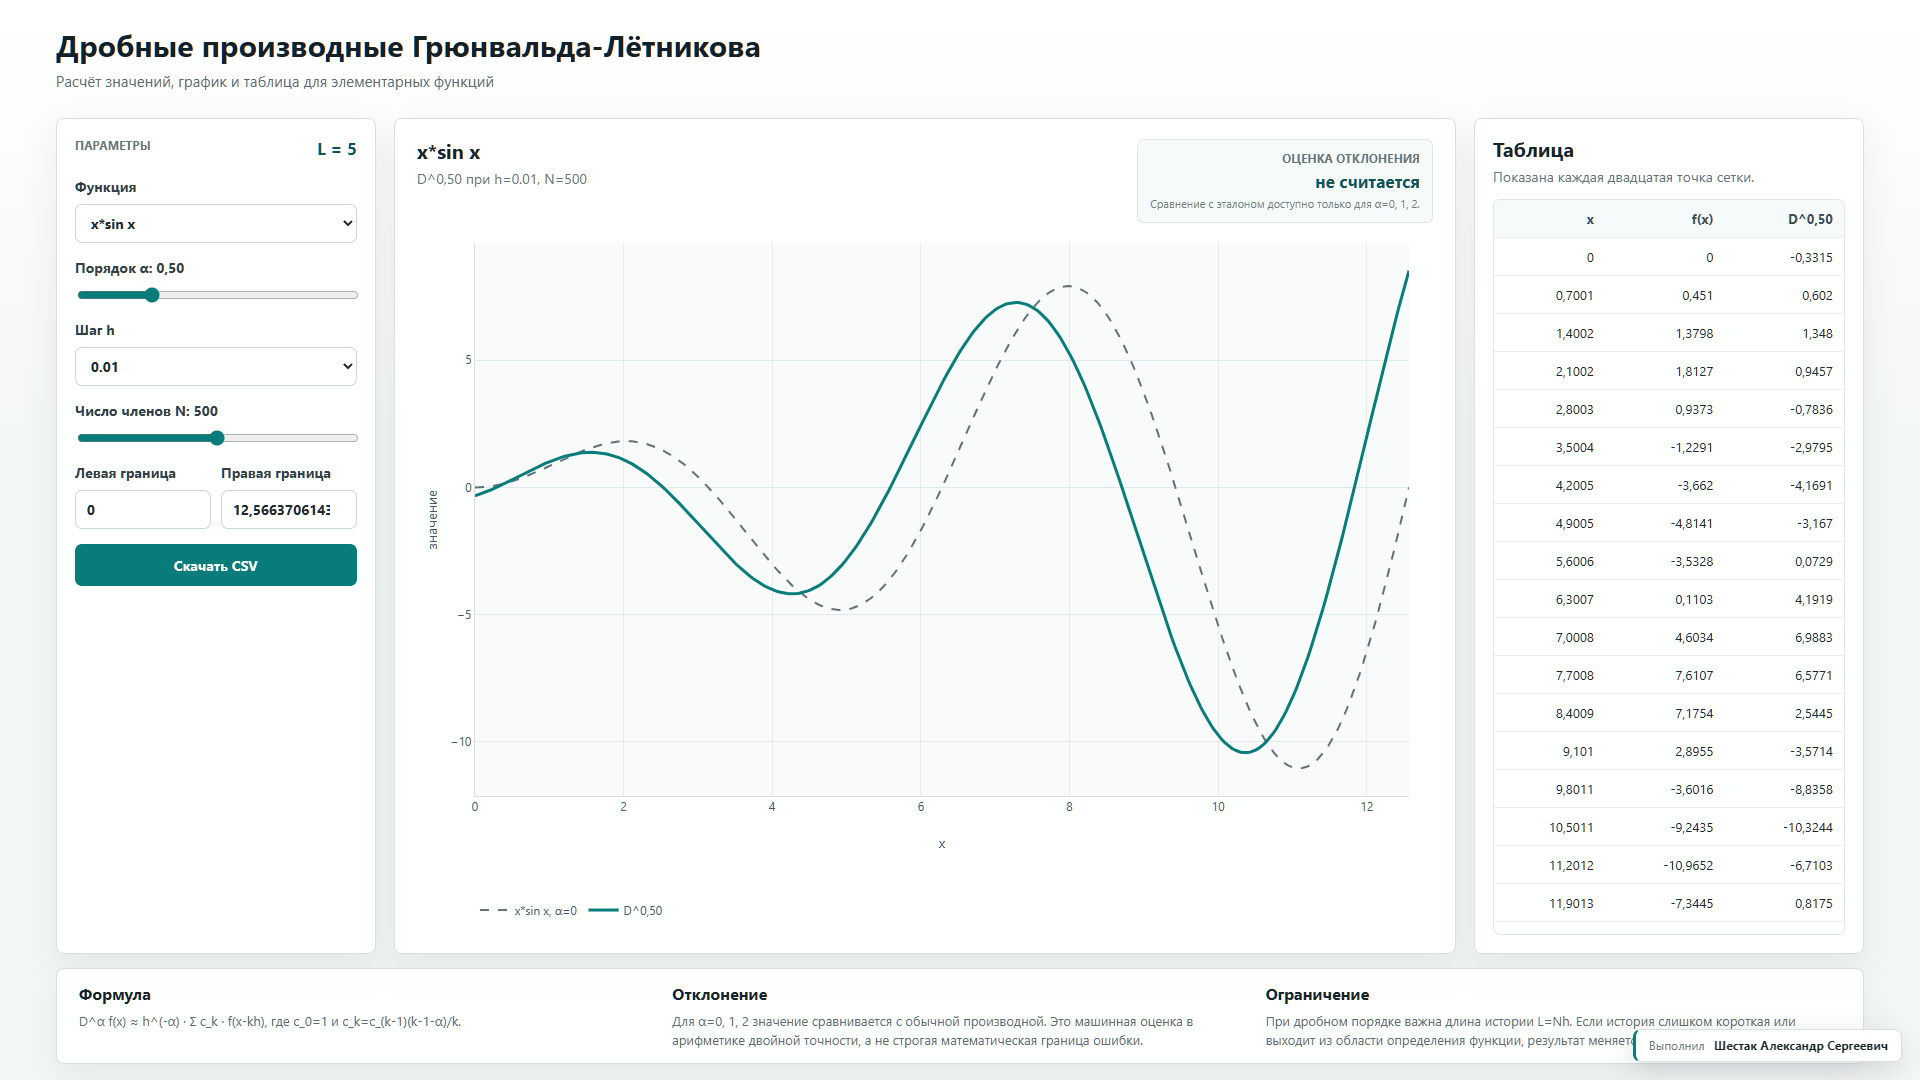
\includegraphics[width=0.95\textwidth]{web_ui.png}
\caption{Веб-интерфейс программы с параметрами метода, интерактивным графиком Plotly и таблицей значений}
\label{fig:ui}
\end{figure}

\subsection{Тестирование программы}

Корректность реализации контролируется на свойствах, которые не зависят от конкретной функции, и на сравнении с известными производными (таблица~\ref{tab:tests}). Эти проверки оформлены как автоматические тесты в каталоге \texttt{tests/} и запускаются командой \texttt{pytest} из корня проекта. Влияние округления при малом $h$ дополнительно рассматривается в разделе~\ref{sec:floor}. Тесты не доказывают корректность полностью, но ловят грубые ошибки, включая неверный знак, забытое деление на $h^{\alpha}$, неправильный порядок точек и ошибку в рекуррентной формуле.

\begin{table}[htbp]
\centering
\caption{Проверки реализации}
\label{tab:tests}
\begin{tabular}{|L{4.3cm}|L{3.6cm}|L{4.4cm}|}
\hline
Тест & Ожидаемый результат & Что проверяет \\
\hline
$\alpha=0$. & $\D^0 f = f$. & Базовую нормировку. \\
\hline
$\alpha=1$, $\sin x$. & Близко к $\cos x$. & Знак и деление на $h$. \\
\hline
$\alpha=2$, $x^2$. & Ровно $2$. & Коэффициенты второго порядка. \\
\hline
$\alpha=0{,}5$, $x^2$, $a=0$. & Формула через $\Gamma$. & Дробный порядок. \\
\hline
Сумма коэффициентов. & Стремится к нулю. & Рекуррентную формулу. \\
\hline
$\ln x$ при выходе за область. & \texttt{NaN}. & Обработку области определения. \\
\hline
Малый шаг $h$. & Рост ошибки. & Влияние округления. \\
\hline
Ячейки сводной таблицы. & Совпадают с $\Gamma$-формулой. & Композицию схем в \texttt{master\_table}. \\
\hline
\end{tabular}
\end{table}

\section{Вычислительные эксперименты}

\subsection{Сводная таблица дробных производных элементарных функций}
\label{sec:master}

Главным результатом работы стала собранная численным методом таблица дробных производных элементарных функций (таблица~\ref{tab:master}). По строкам в ней идут функции из набора \texttt{functions.py}, по столбцам отложены порядки $\alpha=0,\,0{,}5,\,1,\,1{,}5,\,2$, а в ячейке стоит значение $\D^{\alpha}f$ в опорной точке $x_0$, посчитанное по формуле~\eqref{eq:gl-num}. Каждая функция взята в своём естественном режиме (раздел~\ref{sec:regimes}). Степенные считаются с нижним пределом $a=0$, остальные с конечной памятью $L=Nh=5$ (для $\tan x$ короче, $L=1$). Замкнутые формы для тех же функций собраны в справочной таблице~\ref{tab:reftable}. Численная схема воспроизводит их строка за строкой, а вся остальная часть главы показывает, почему её числам можно верить.

\begin{table}[htbp]
\centering
\caption{Сводная таблица численных дробных производных $\D^{\alpha}f$ элементарных функций по Грюнвальду--Летникову ($h=0{,}01$)}
\label{tab:master}
\small
\begin{tabular}{|l|c|l|r|r|r|r|r|}
\hline
$f(x)$ & $x_0$ & Режим & $\D^{0}$ & $\D^{0{,}5}$ & $\D^{1}$ & $\D^{1{,}5}$ & $\D^{2}$ \\
\hline
$1$            & $2$ & $a=0$        & $1{,}000$ & $0{,}399$  & $0{,}000$  & $-0{,}100$ & $0{,}000$ \\
\hline
$x$            & $2$ & $a=0$        & $2{,}000$ & $1{,}595$  & $1{,}000$  & $0{,}400$  & $0{,}000$ \\
\hline
$x^2$          & $2$ & $a=0$        & $4{,}000$ & $4{,}247$  & $3{,}990$  & $3{,}186$  & $2{,}000$ \\
\hline
$x^3$          & $2$ & $a=0$        & $8{,}000$ & $10{,}181$ & $11{,}940$ & $12{,}694$ & $11{,}940$ \\
\hline
$e^{x}$        & $1$ & память $L=5$  & $2{,}718$ & $2{,}712$  & $2{,}705$  & $2{,}698$  & $2{,}691$ \\
\hline
$\sin x$       & $1$ & память $L=5$  & $0{,}841$ & $0{,}997$  & $0{,}545$  & $-0{,}212$ & $-0{,}836$ \\
\hline
$\cos x$       & $1$ & память $L=5$  & $0{,}540$ & $-0{,}197$ & $-0{,}839$ & $-0{,}982$ & $-0{,}549$ \\
\hline
$\sin x+\cos x$& $1$ & память $L=5$  & $1{,}382$ & $0{,}800$  & $-0{,}294$ & $-1{,}193$ & $-1{,}385$ \\
\hline
$\ln x$        & $8$ & память $L=5$  & $2{,}079$ & $0{,}705$  & $0{,}125$  & $-0{,}023$ & $-0{,}016$ \\
\hline
$x\sin x$      & $1$ & память $L=5$  & $0{,}841$ & $1{,}011$  & $1{,}381$  & $1{,}287$  & $0{,}270$ \\
\hline
$xe^{x}$       & $1$ & память $L=5$  & $2{,}718$ & $4{,}059$  & $5{,}396$  & $6{,}725$  & $8{,}047$ \\
\hline
$\tan x$\textsuperscript{*} & $1$ & память $L=1$  & $1{,}557$ & $2{,}287$  & $3{,}373$  & $5{,}418$  & $10{,}125$ \\
\hline
\end{tabular}

\vspace{2pt}
{\footnotesize\raggedright\textsuperscript{*}\,Строка $\tan x$ дана как иллюстрация роста вблизи разрыва $\pi/2$: замкнутого эталона у неё нет, и само число зависит от выбранной памяти.\par}
\end{table}

Прежде чем разбирать числа, стоит объяснить, почему режим у строк разный. Сделано это намеренно. Единого нижнего предела, при котором у всех перечисленных функций сразу нашлась бы замкнутая элементарная форма для сверки, попросту не существует. При $a=0$ степенные функции дают чистую формулу через гамма-функцию~\eqref{eq:power}, но у $\sin x$, $\cos x$ и $e^x$ от того же предела появляется начальный переходный член, и простого фазового сдвига уже нет. В форме Лиувилля ($a\to-\infty$), наоборот, фазовые формулы~\eqref{eq:trig} для тригонометрии и экспоненты точны, зато степенная сумма по бесконечной истории расходится, ведь слагаемые $(x-kh)^{\beta}$ растут быстрее, чем убывают коэффициенты. Поэтому каждая функция взята в единственном режиме, где у неё есть чистый аналитический эталон. Режим выписан отдельным столбцом, а сверка каждой ячейки со своей замкнутой формой вынесена в таблицу~\ref{tab:masterref}. По сути таблица~\ref{tab:master} собрана как численный атлас, где каждая строка взята в своём, естественном для функции режиме. Тот же оператор можно применить ко всем функциям и с общим пределом $a=0$, и тогда тригонометрия и экспонента заметно отходят от фазовых формул. Такой единый расчёт приведён в приложении (таблица~\ref{tab:mastera0}). Он показывает, что разные режимы в основной таблице выбраны ради удобной сверки с эталонами, а сам метод одинаково считает все функции.

Там, где эталонная формула есть, таблица с ней согласуется. Полная сверка для двух дробных порядков собрана в таблице~\ref{tab:masterref}. Для степенных функций значения в режиме $a=0$ совпадают с формулой~\eqref{eq:power} через гамма-функцию. При $\alpha=0{,}5$ численные $4{,}247$ ($x^2$), $1{,}595$ ($x$) и $10{,}181$ ($x^3$) отвечают точным $4{,}255$, $1{,}596$ и $10{,}213$, с отклонением порядка $h$. Производная постоянной при дробном $\alpha$ нулю не равна. Значение $\D^{0{,}5}1=0{,}399$ отвечает $x^{-\alpha}/\Gamma(1-\alpha)$ и сразу выдаёт память метода. Для $\sin x$, $\cos x$ и их суммы столбец $\alpha=1$ даёт почти точную первую производную ($\D^1\sin x|_{x=1}=0{,}545$ против $\cos 1=0{,}540$), а дробные столбцы приближают фазовые формулы~\eqref{eq:trig} с поправкой на конечную историю. Именно эта поправка и видна в таблице~\ref{tab:masterref}. У тригонометрии и $e^x$ остаётся зазор порядка процента от амплитуды, тогда как степенные в режиме $a=0$ ложатся на эталон почти точно. Строки $\ln x$, $\tan x$, $x\sin x$, $xe^x$ замкнутой формулы не имеют и приводятся только численно. У $\tan x$ значения быстро растут с $\alpha$ из-за близости разрыва.

\begin{table}[htbp]
\centering
\caption{Сверка сводной таблицы~\ref{tab:master} с замкнутыми формами (точки $x_0$ те же). Эталон для степенных задаёт формула~\eqref{eq:power} через $\Gamma$ в режиме $a=0$, для остальных его роль играет форма Лиувилля~\eqref{eq:trig}; зазор у $\sin x$, $\cos x$ и $e^x$ отражает конечную память $L=5$}
\label{tab:masterref}
\small
\begin{tabular}{|l|r|r|r|r|}
\hline
$f(x)$ & числ. $\D^{0{,}5}$ & замкн. $\D^{0{,}5}$ & числ. $\D^{1{,}5}$ & замкн. $\D^{1{,}5}$ \\
\hline
$1$            & $0{,}399$  & $0{,}399$  & $-0{,}100$ & $-0{,}100$ \\
\hline
$x$            & $1{,}595$  & $1{,}596$  & $0{,}400$  & $0{,}399$ \\
\hline
$x^2$          & $4{,}247$  & $4{,}255$  & $3{,}186$  & $3{,}192$ \\
\hline
$x^3$          & $10{,}181$ & $10{,}213$ & $12{,}694$ & $12{,}766$ \\
\hline
$e^{x}$        & $2{,}712$  & $2{,}718$  & $2{,}698$  & $2{,}718$ \\
\hline
$\sin x$       & $0{,}997$  & $0{,}977$  & $-0{,}212$ & $-0{,}213$ \\
\hline
$\cos x$       & $-0{,}197$ & $-0{,}213$ & $-0{,}982$ & $-0{,}977$ \\
\hline
$\sin x+\cos x$& $0{,}800$  & $0{,}764$  & $-1{,}193$ & $-1{,}190$ \\
\hline
\end{tabular}
\end{table}

Дальше каждый столбец и каждая строка этой таблицы разбираются по отдельности. Это переход формы при росте $\alpha$, проверка целых порядков, влияние шага $h$ и числа членов $N$, оценки точности и устойчивости. По сути вся глава обосновывает, что значениям таблицы~\ref{tab:master} можно верить.

\subsection{План экспериментов}

В основной части рассматриваются функции $x$, $x^2$, $\sin x$, $\cos x$, $e^x$, а в качестве расширения берутся $\ln x$, $x^3$ и комбинированные функции $x\sin x$, $x e^x$, $\sin x+\cos x$. Все они зарегистрированы в \texttt{functions.py} и доступны как из командной строки, так и в интерфейсе. Их таблицы сохраняются в каталог \texttt{tables/} (например, $x\sin x$ попадает в \texttt{xsin\_values.csv}). Если не сказано иное, базовые параметры $h=0{,}01$, $N=500$.

Набор функций подобран не случайно. Главным требованием был аналитический эталон хотя бы в одном режиме. Степенные $x$, $x^2$, $x^3$ дают строгую сверку через гамма-формулу~\eqref{eq:power}, для $\sin x$, $\cos x$ и $e^x$ работают фазовые формулы~\eqref{eq:trig} в форме Лиувилля, а целые порядки любой функции сверяются с классической производной. Дальше хотелось охватить разные типы поведения, чтобы на таблице были видны и согласие с эталоном, и границы метода. Сюда вошли ограниченные колебания $\sin x$ и $\cos x$ и, для контраста, быстро растущие $e^x$ и $x^3$. Добавлены и два неудобных для метода случая. У $\ln x$ область определения ограничена снизу, а $\tan x$ и вовсе имеет разрыв. Простейшие же комбинации $x\sin x$, $xe^x$, $\sin x+\cos x$ показывают, что схема работает и там, где замкнутой формулы уже нет, а функция остаётся элементарной. Что-то вроде $\sqrt{x}$ или $a^x$ к этому ничего не добавляет, поэтому в набор не вошло.

Сводка экспериментов приведена в таблице~\ref{tab:plan}.

\begin{table}[htbp]
\centering
\caption{Параметры вычислительных экспериментов}
\label{tab:plan}
\begin{tabular}{|L{4.0cm}|L{4.2cm}|L{4.1cm}|}
\hline
Эксперимент & Функция, $\alpha$ & Эталон \\
\hline
Переход формы по порядку. & $\sin x$, $\alpha=0\dots2$. & $\cos x$, $-\sin x$. \\
\hline
Проверка целых порядков. & $x^2$, $e^x$, $\sin x$, $\cos x$. & Классическая производная. \\
\hline
Влияние шага $h$. & $\sin x$, $\alpha=1$. & $\cos x$. \\
\hline
Влияние числа $N$. & $\sin x$, $\alpha=0{,}5$. & $\sin(x+\pi/4)$. \\
\hline
Сходимость по $h$. & $\sin x$ и $x^2$. & $\cos1$ и формула $\Gamma$. \\
\hline
Степенные функции. & $x^2,x^3$, режим $a=0$. & Формула~\eqref{eq:power}. \\
\hline
\end{tabular}
\end{table}

\subsection{Изменение функции при росте порядка производной}

Проще всего рост порядка читается на $\sin x$, где кривая плавно переходит от исходной функции к её производным (рисунок~\ref{fig:sin}). При $\alpha=0$ это сам $\sin x$, при $\alpha=1$ кривая ложится на $\cos x$, при $\alpha=2$ на $-\sin x$. Промежуточные порядки $\alpha=0{,}5$ и $\alpha=1{,}5$ дают плавный сдвиг фазы. Каждая такая кривая получается как взвешенная сумма значений функции в предыдущих точках. На целых порядках она ложится на пунктирные эталоны $\cos x$ и $-\sin x$.

\begin{figure}[htbp]
\centering
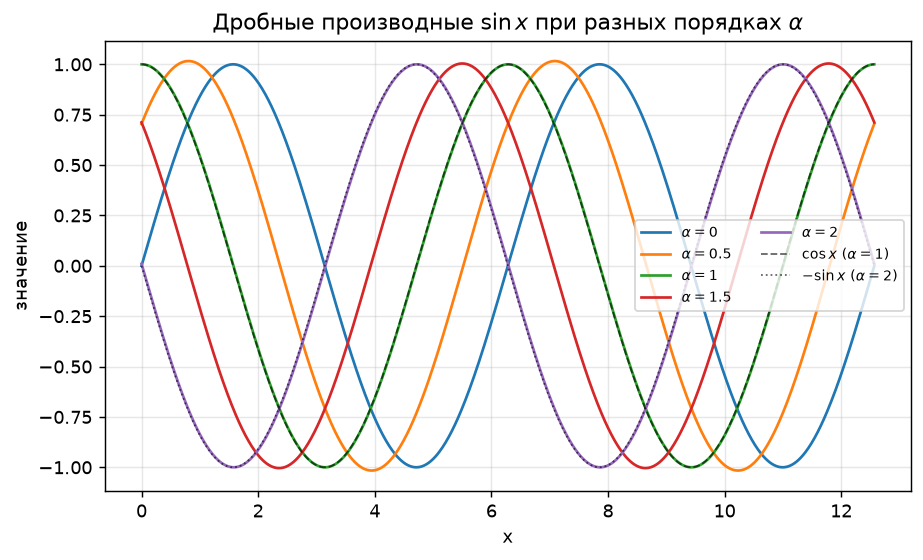
\includegraphics[width=0.85\textwidth]{sin_orders.png}
\caption{Дробные производные $\sin x$ при $\alpha=0,\,0{,}5,\,1,\,1{,}5,\,2$ ($h=0{,}01$, $N=500$); пунктиром показаны эталоны $\cos x$ и $-\sin x$}
\label{fig:sin}
\end{figure}

Те же значения в табличном виде приведены в таблице~\ref{tab:sinval}. В строке $x=\pi/2\approx1{,}571$ видно, как растёт порядок. Здесь $f=1$, при $\alpha=0{,}5$ значение $0{,}732$, при $\alpha=1$ значение $0{,}005$, то есть $\cos(\pi/2)=0$ с точностью до шага. В строке $x=\pi$ значения при $\alpha=0{,}5$ и $0{,}75$ отрицательные, так как фаза уже ушла за $\cos x$ к $-\sin x$.

\begin{table}[htbp]
\centering
\caption{Значения дробной производной $\sin x$ при $h=0{,}01$, $N=500$}
\label{tab:sinval}
\begin{tabular}{|r|r|r|r|r|r|}
\hline
$x$ & $f(x)$ & $\D^{0{,}25}$ & $\D^{0{,}5}$ & $\D^{0{,}75}$ & $\D^{1}$ \\
\hline
$0{,}000$ & $0{,}000$ & $0{,}380$ & $0{,}705$ & $0{,}923$ & $1{,}000$ \\
\hline
$0{,}785$ & $0{,}707$ & $0{,}940$ & $1{,}016$ & $0{,}933$ & $0{,}711$ \\
\hline
$1{,}571$ & $1{,}000$ & $0{,}950$ & $0{,}732$ & $0{,}397$ & $0{,}005$ \\
\hline
$2{,}356$ & $0{,}707$ & $0{,}403$ & $0{,}020$ & $-0{,}371$ & $-0{,}704$ \\
\hline
$3{,}142$ & $0{,}000$ & $-0{,}380$ & $-0{,}705$ & $-0{,}923$ & $-1{,}000$ \\
\hline
$4{,}712$ & $-1{,}000$ & $-0{,}950$ & $-0{,}732$ & $-0{,}397$ & $-0{,}005$ \\
\hline
$6{,}283$ & $0{,}000$ & $0{,}380$ & $0{,}705$ & $0{,}923$ & $1{,}000$ \\
\hline
\end{tabular}
\end{table}

Этот плавный переход не останавливается на $\alpha=1$. С дальнейшим ростом порядка фаза уезжает ещё сильнее, и к $\alpha=2$ кривая садится на $-\sin x$ (таблица~\ref{tab:sinval-high}). В точке $x=\pi/2$ значение монотонно опускается от $1$ при $\alpha=0$ до $-1$ при $\alpha=2$, проходя через ноль около $\alpha=1$.

\begin{table}[htbp]
\centering
\caption{Значения дробной производной $\sin x$ для верхних порядков, $h=0{,}01$, $N=500$}
\label{tab:sinval-high}
\begin{tabular}{|r|r|r|r|r|r|}
\hline
$x$ & $f(x)$ & $\D^{1{,}25}$ & $\D^{1{,}5}$ & $\D^{1{,}75}$ & $\D^{2}$ \\
\hline
$0{,}000$ & $0{,}000$ & $0{,}926$ & $0{,}712$ & $0{,}390$ & $0{,}010$ \\
\hline
$0{,}785$ & $0{,}707$ & $0{,}384$ & $0{,}002$ & $-0{,}378$ & $-0{,}700$ \\
\hline
$1{,}571$ & $1{,}000$ & $-0{,}383$ & $-0{,}708$ & $-0{,}924$ & $-1{,}000$ \\
\hline
$2{,}356$ & $0{,}707$ & $-0{,}925$ & $-1{,}004$ & $-0{,}929$ & $-0{,}714$ \\
\hline
$3{,}142$ & $0{,}000$ & $-0{,}926$ & $-0{,}712$ & $-0{,}390$ & $-0{,}010$ \\
\hline
$4{,}712$ & $-1{,}000$ & $0{,}383$ & $0{,}708$ & $0{,}924$ & $1{,}000$ \\
\hline
$6{,}283$ & $0{,}000$ & $0{,}926$ & $0{,}712$ & $0{,}390$ & $0{,}010$ \\
\hline
\end{tabular}
\end{table}

\subsection{Проверка на целых порядках}

Целые порядки удобны тем, что ответ известен заранее. При $\alpha=1$ и $\alpha=2$ численный результат можно положить рядом с обычной производной и сразу увидеть расхождение. Для четырёх функций такое сравнение $\D^1$ с точной первой производной, вместе с абсолютной и относительной ошибками, собрано в таблице~\ref{tab:cmp}.

\begin{table}[htbp]
\centering
\caption{Сравнение $\D^1$ с классической первой производной, $h=0{,}01$, $N=500$}
\label{tab:cmp}
\begin{tabular}{|l|r|r|r|r|r|}
\hline
Функция & $x$ & ГЛ & Точная & Абс. ошибка & Отн. ошибка \\
\hline
$x^2$ & $2{,}3$ & $4{,}590$ & $4{,}600$ & $0{,}010$ & $0{,}0022$ \\
\hline
$x^2$ & $5{,}0$ & $9{,}990$ & $10{,}000$ & $0{,}010$ & $0{,}0010$ \\
\hline
$e^x$ & $0{,}5$ & $1{,}641$ & $1{,}649$ & $0{,}008$ & $0{,}0050$ \\
\hline
$e^x$ & $5{,}0$ & $147{,}674$ & $148{,}413$ & $0{,}740$ & $0{,}0050$ \\
\hline
$\sin x$ & $1{,}4$ & $0{,}175$ & $0{,}170$ & $0{,}005$ & $0{,}0049$ \\
\hline
$\cos x$ & $3{,}2$ & $0{,}053$ & $0{,}058$ & $0{,}005$ & $0{,}0050$ \\
\hline
\end{tabular}
\end{table}

Для $x^2$ абсолютная ошибка ровно $0{,}010$ в каждой точке. Левая разность даёт $\frac{x^2-(x-h)^2}{h}=2x-h$, поэтому появляется систематический сдвиг на $h=0{,}01$. Для $\sin x$ и $\cos x$ ошибка около $0{,}005$, порядка $h/2$. Для $e^x$ абсолютная ошибка растёт вместе с функцией, от $0{,}008$ при $x=0{,}5$ до $0{,}74$ при $x=5$, но относительная держится около $0{,}005$. Для сравнения разных функций это и важно, ведь одна абсолютная ошибка мало о чём говорит, и ориентируются на относительную. У самого столбца относительной ошибки есть оговорка. Для $\sin x$ и $\cos x$ здесь $|g|<1$, знаменатель $\max(1,|g|)$ обращается в единицу, и приведённое число совпадает с абсолютной ошибкой. Как настоящая относительная оно читается только для $e^x$ при больших $x$, где $|g|\geqslant1$. На рисунке~\ref{fig:check} тот же тест показан графически.

\begin{figure}[htbp]
\centering
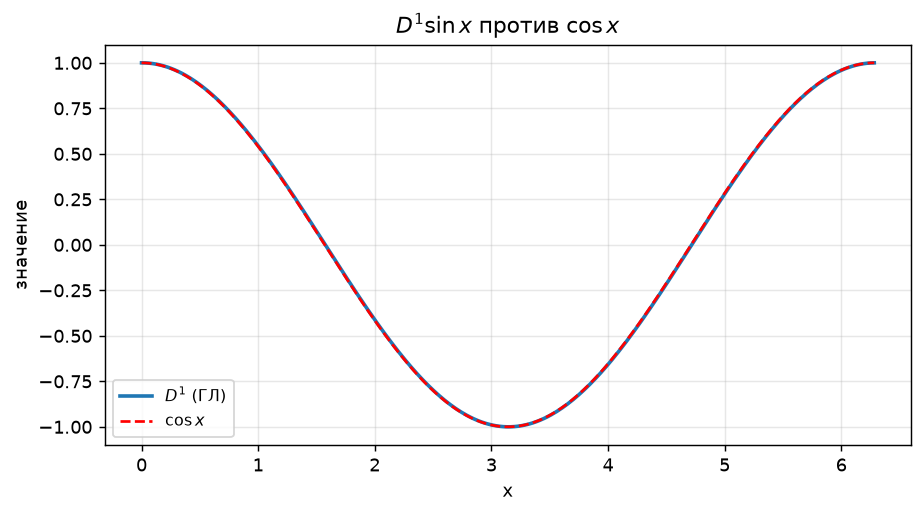
\includegraphics[width=0.8\textwidth]{alpha1_check.png}
\caption{$\D^1\sin x$ по Грюнвальду--Летникову приближает $\cos x$ с ошибкой порядка $h$ ($h=0{,}01$, $N=500$)}
\label{fig:check}
\end{figure}

Для $\alpha=2$ на $x^2$ результат равен ровно $2{,}000$ во всех точках независимо от $h$: вторая разность квадратичной функции точна. Независимость от шага делает этот случай надёжной эталонной проверкой.

\subsection{Влияние шага $h$}
\label{sec:h}

Чем крупнее шаг $h$, тем дальше $\D^1\sin x$ отходит от эталона $\cos x$. Эту зависимость собирает таблица~\ref{tab:h} ($N=500$).

\begin{table}[htbp]
\centering
\caption{Влияние шага $h$ на ошибку $\D^1\sin x$ ($N=500$)}
\label{tab:h}
\begin{tabular}{|r|r|r|r|}
\hline
$h$ & $L=Nh$ & Макс. ошибка & Сред. ошибка \\
\hline
$0{,}100$ & $50{,}0$ & $0{,}0500$ & $0{,}0335$ \\
\hline
$0{,}050$ & $25{,}0$ & $0{,}0250$ & $0{,}0167$ \\
\hline
$0{,}020$ & $10{,}0$ & $0{,}0100$ & $0{,}0067$ \\
\hline
$0{,}010$ & $5{,}0$  & $0{,}0050$ & $0{,}0033$ \\
\hline
$0{,}005$ & $2{,}5$  & $0{,}0025$ & $0{,}0017$ \\
\hline
$0{,}001$ & $0{,}5$  & $0{,}0005$ & $0{,}0003$ \\
\hline
\end{tabular}
\end{table}

Зависимость получается почти линейной. При уменьшении $h$ вдвое ошибка падает вдвое, максимальная ошибка примерно равна $h/2$. При $h=0{,}1$ максимальная ошибка $0{,}05$, при $h=0{,}01$ уже $0{,}005$, в десять раз меньше. На рисунке~\ref{fig:h} при $h=0{,}5$ кривая заметно сдвинута и ниже по амплитуде, при $h=0{,}02$ почти сливается с эталоном.

\begin{figure}[htbp]
\centering
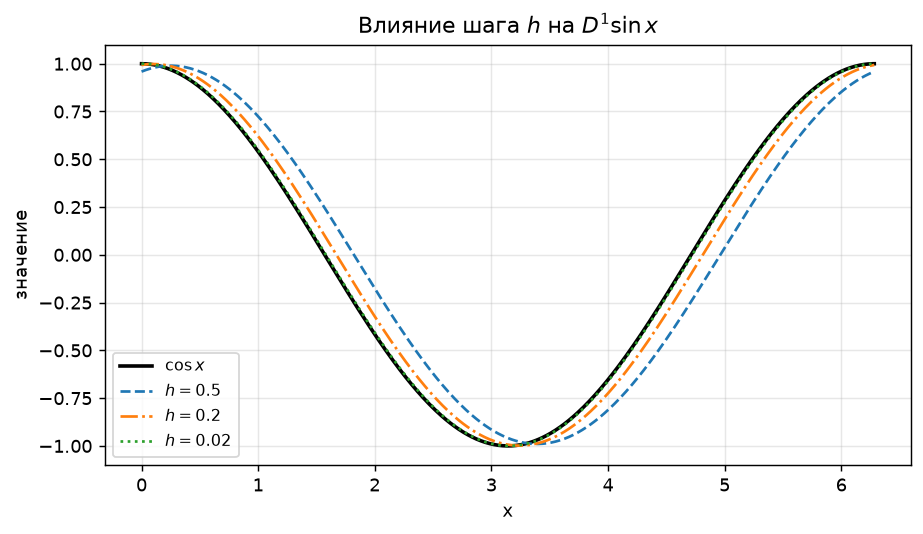
\includegraphics[width=0.8\textwidth]{h_influence.png}
\caption{Влияние шага $h$ на $\D^1\sin x$ при разной плотности сетки ($N=500$)}
\label{fig:h}
\end{figure}

\subsection{Влияние числа членов $N$}
\label{sec:N}

Насколько длинной должна быть история? Для целого порядка вопрос не стоит, там работают всего два коэффициента. Для дробного же число членов $N$ определяет точность напрямую. В таблице~\ref{tab:N} оно растёт от $5$ до $1000$ при $\sin x$, $\alpha=0{,}5$ и $h=0{,}01$, а эталоном служит $\sin(x+\pi/4)$.

\begin{table}[htbp]
\centering
\caption{Влияние числа членов $N$ на ошибку $\D^{0{,}5}\sin x$ ($h=0{,}01$)}
\label{tab:N}
\begin{tabular}{|r|r|r|r|}
\hline
$N$ & $L=Nh$ & Макс. ошибка & Сред. ошибка \\
\hline
$5$    & $0{,}05$ & $1{,}850$ & $1{,}175$ \\
\hline
$20$   & $0{,}20$ & $0{,}719$ & $0{,}458$ \\
\hline
$50$   & $0{,}50$ & $0{,}336$ & $0{,}214$ \\
\hline
$100$  & $1{,}00$ & $0{,}170$ & $0{,}109$ \\
\hline
$300$  & $3{,}00$ & $0{,}044$ & $0{,}028$ \\
\hline
$500$  & $5{,}00$ & $0{,}025$ & $0{,}016$ \\
\hline
$1000$ & $10{,}0$ & $0{,}008$ & $0{,}005$ \\
\hline
\end{tabular}
\end{table}

При $N=5$ (история $L=0{,}05$) ошибка достигает $1{,}85$, потому что сумма обрывается раньше, чем накапливается память функции. С ростом $N$ ошибка падает медленно. $N=100$ даёт $0{,}17$, $N=500$ даёт $0{,}025$, $N=1000$ даёт $0{,}008$. Причина в медленном затухании коэффициентов $|c_k|\sim k^{-1{,}5}$. Падение не бесконечно. При фиксированном $h$ рост $N$ убирает только ошибку усечения, а под ней остаётся ошибка дискретизации порядка $h$ (раздел~\ref{sec:order}), и именно в эту полку упёрлась бы таблица при дальнейшем росте $N$. На рисунке~\ref{fig:N} при $N=5$ кривая не похожа на эталон, при $N=20$ уже близка, при $N=200$ почти ложится на $\sin(x+\pi/4)$.

\begin{figure}[htbp]
\centering
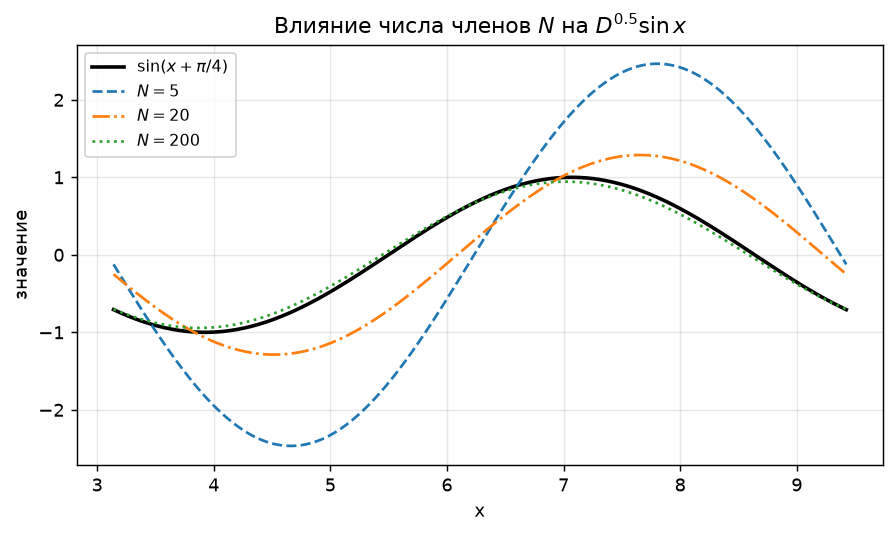
\includegraphics[width=0.8\textwidth]{N_influence.png}
\caption{Влияние числа членов $N$ на $\D^{0{,}5}\sin x$ ($h=0{,}01$)}
\label{fig:N}
\end{figure}

Уменьшать ошибку для дробного порядка только шагом $h$ недостаточно. При короткой истории $Nh$ мелкий шаг не помогает.

\subsection{Память метода}
\label{sec:memory}

Затухание коэффициентов объясняет разное поведение целого и дробного порядка (рисунок~\ref{fig:mem}). На лог-лог графике коэффициенты при $\alpha=0{,}5$ ложатся на прямую с наклоном $-1{,}5=-(\alpha+1)$. При $\alpha=1{,}5$ наклон круче, память короче. При целом $\alpha=1$ ненулевой коэффициент всего один, и памяти нет.

\begin{figure}[htbp]
\centering
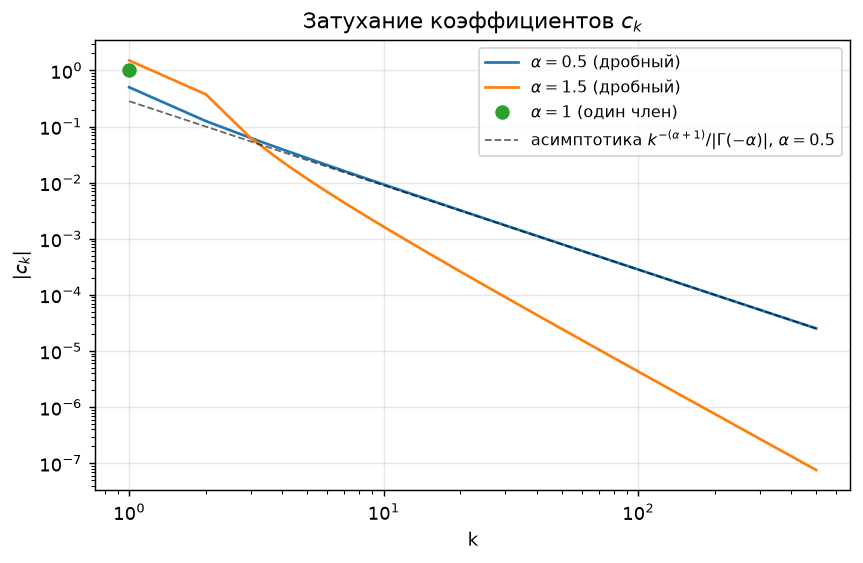
\includegraphics[width=0.8\textwidth]{coeff_decay.png}
\caption{Затухание коэффициентов $|c_k|$ для дробного и целого порядка}
\label{fig:mem}
\end{figure}

\subsection{Сходимость и порядок точности}
\label{sec:conv}

Для оценки порядка точности измерялось падение ошибки при уменьшении $h$ в фиксированной точке. Для $\sin x$, $\alpha=1$, $x=1$ эталон $\cos1\approx0{,}5403$ (таблица~\ref{tab:conv}).

\begin{table}[htbp]
\centering
\caption{Сходимость по $h$ для $\D^1\sin x$ в точке $x=1$}
\label{tab:conv}
\begin{tabular}{|r|r|r|}
\hline
$h$ & Ошибка & Отношение \\
\hline
$0{,}200$  & $0{,}0803$ & --- \\
\hline
$0{,}100$  & $0{,}0411$ & $1{,}95$ \\
\hline
$0{,}050$  & $0{,}0208$ & $1{,}98$ \\
\hline
$0{,}025$  & $0{,}0105$ & $1{,}99$ \\
\hline
$0{,}0125$ & $0{,}0052$ & $1{,}99$ \\
\hline
$0{,}00625$& $0{,}0026$ & $2{,}00$ \\
\hline
\end{tabular}
\end{table}

При уменьшении шага вдвое ошибка падает примерно вдвое (отношение $\approx2$), то есть метод имеет первый порядок точности, $O(h)$. Это согласуется с известными результатами о порядке аппроксимации дискретного дробного исчисления \cite{lubich, meerschaert, dfff}. На рисунке~\ref{fig:conv} обе зависимости (для $\sin x$ при $\alpha=1$ и для $x^2$ при $\alpha=0{,}5$ в режиме $a=0$) ложатся в прямые с наклоном $1$. Дробный случай ведёт себя так же, как целый, что подтверждает корректность реализации для дробного порядка.

\begin{figure}[htbp]
\centering
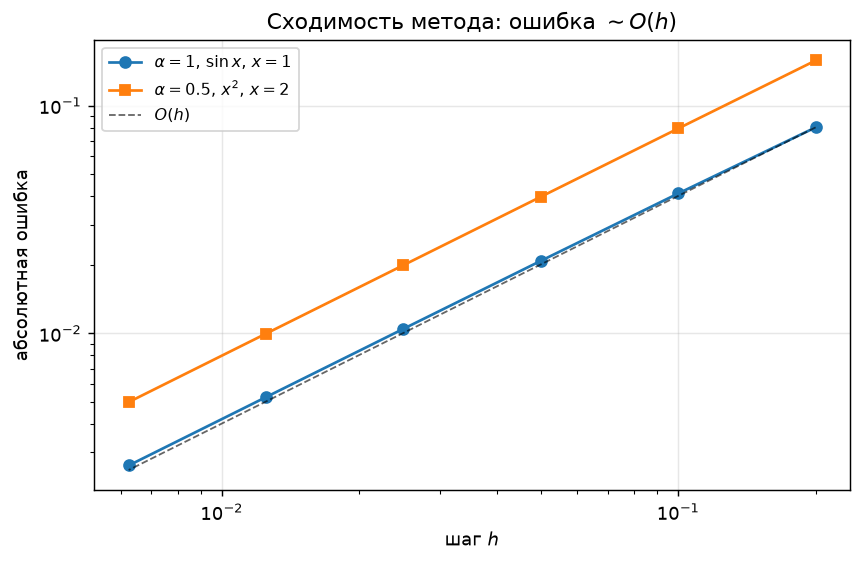
\includegraphics[width=0.8\textwidth]{convergence.png}
\caption{Сходимость по шагу $h$ для целого и дробного порядка}
\label{fig:conv}
\end{figure}

\subsection{Степенные функции и логарифм}

Для $x^2$ дробная производная в режиме $a=0$ показана на рисунке~\ref{fig:pow}. При $\alpha=0{,}5$ численная кривая ложится на формулу через гамма-функцию, при $\alpha=1$ приближает $2x$ с систематическим сдвигом левой разности.

\begin{figure}[htbp]
\centering
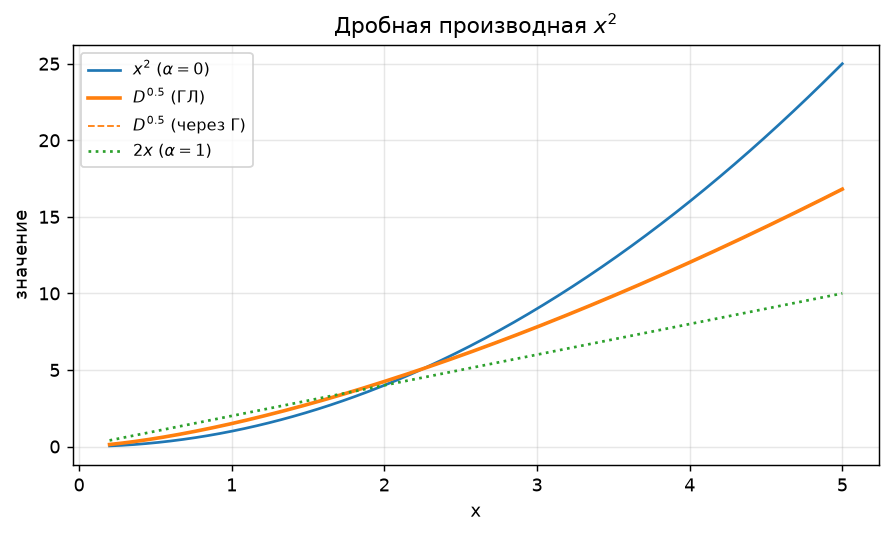
\includegraphics[width=0.8\textwidth]{power_frac.png}
\caption{Дробная производная $x^2$ в режиме $a=0$ при нескольких порядках $\alpha$ ($h=0{,}01$)}
\label{fig:pow}
\end{figure}

Для $x^3$ закономерность степенных функций сохраняется (рисунок~\ref{fig:x3}, таблица~\ref{tab:x3}). Расчёт ведётся в режиме $a=0$. При $\alpha=2$ получаются значения вида $6x-0{,}06$. Точная вторая производная равна $6x$, а сдвиг $0{,}06=6h$ появляется потому, что для кубической функции вторая разность уже не точна. При $\alpha=1$ результат равен $3x^2-3xh+h^2$. Дробный порядок $\D^{0{,}5}$ согласуется с формулой~\eqref{eq:power}. При $x=1$ значение $1{,}794$ близко к точному $\Gamma(4)/\Gamma(3{,}5)\approx1{,}805$.

\begin{table}[htbp]
\centering
\caption{Значения дробной производной $x^3$ в режиме $a=0$ при $N=\lfloor x/h\rfloor$ и $h=0{,}01$}
\label{tab:x3}
\begin{tabular}{|r|r|r|r|r|r|}
\hline
$x$ & $f(x)$ & $\D^{0{,}5}$ & $\D^{1}$ & $\D^{1{,}5}$ & $\D^{2}$ \\
\hline
$1{,}0$ & $1{,}000$  & $1{,}794$  & $2{,}970$  & $4{,}463$  & $5{,}94$ \\
\hline
$2{,}0$ & $8{,}000$  & $10{,}181$ & $11{,}940$ & $12{,}694$ & $11{,}94$ \\
\hline
$3{,}0$ & $27{,}000$ & $28{,}085$ & $26{,}910$ & $23{,}365$ & $17{,}94$ \\
\hline
$4{,}0$ & $64{,}000$ & $57{,}683$ & $47{,}880$ & $36{,}007$ & $23{,}94$ \\
\hline
\end{tabular}
\end{table}

\begin{figure}[htbp]
\centering
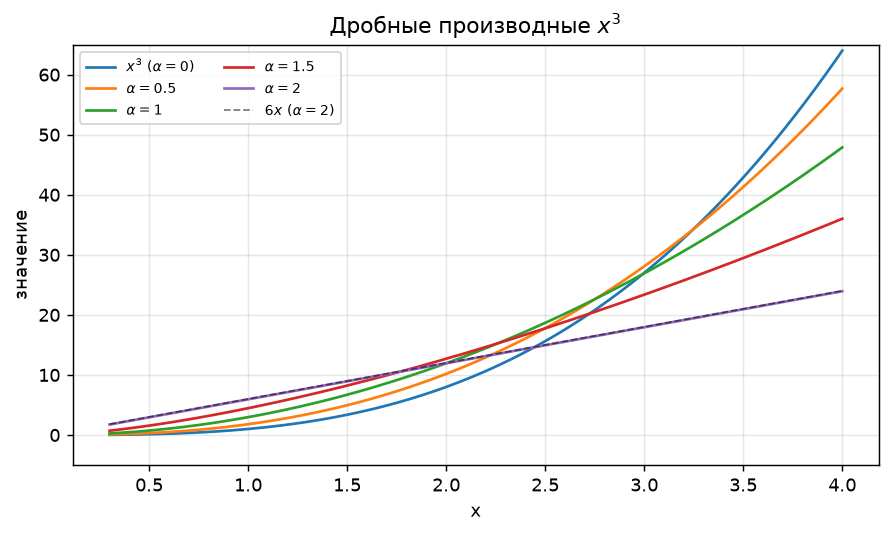
\includegraphics[width=0.8\textwidth]{x3_orders.png}
\caption{Дробные производные $x^3$ при росте порядка $\alpha$ (режим $a=0$, $h=0{,}01$)}
\label{fig:x3}
\end{figure}

Логарифм даёт пример функции с ограниченной областью (рисунок~\ref{fig:ln}). На $[6,10]$ при $h=0{,}01$, $N=500$ условие $x-Nh>0$ выполнено, и $\D^1\ln x$ ложится на $1/x$. Ближе к нулю часть точек $x-kh$ ушла бы в неположительную область, из-за чего отрезок и держат правее.

\begin{figure}[htbp]
\centering
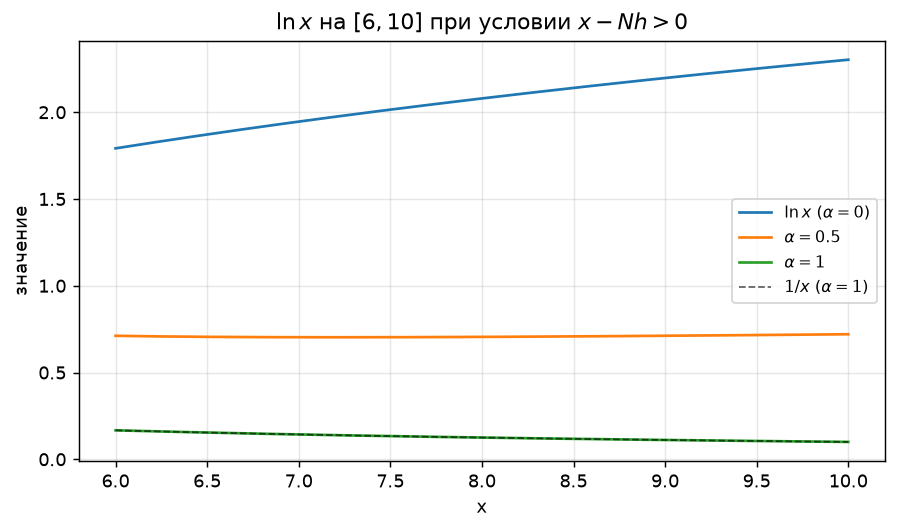
\includegraphics[width=0.8\textwidth]{ln_orders.png}
\caption{Дробная производная $\ln x$ на отрезке $[6,10]$, где выполнено условие $x-Nh>0$ ($h=0{,}01$, $N=500$)}
\label{fig:ln}
\end{figure}

\subsection{Экспонента, левая и правая схемы, касательная}

Для $e^x$ форма при разных $\alpha$ почти не меняется (рисунок~\ref{fig:exp}): все кривые близки к экспоненте, так как $\D^{\alpha}e^x=e^x$ в форме Лиувилля. Интервал здесь взят умеренный, $[0,3]$, и причина чисто практическая. При больших $x$ значения растут так быстро, что абсолютная ошибка перестаёт быть маленькой.

\begin{figure}[htbp]
\centering
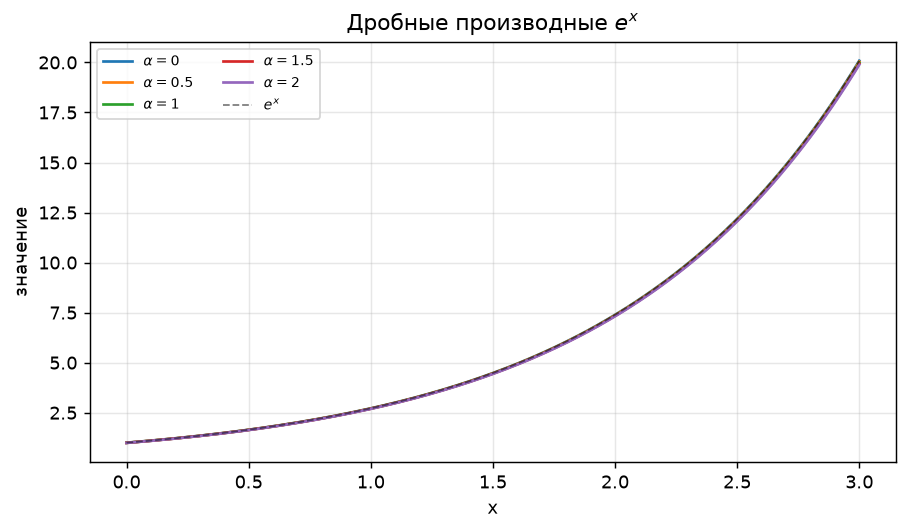
\includegraphics[width=0.8\textwidth]{exp_orders.png}
\caption{Дробные производные $e^x$ почти совпадают с самой функцией ($h=0{,}01$, $N=500$)}
\label{fig:exp}
\end{figure}

Выбор левой схемы заложен в постановку задачи. На рисунке~\ref{fig:lr} для $\sin x$ при $\alpha=0{,}5$ левая производная ложится на $\sin(x+\pi/4)$, а правая на $\sin(x-\pi/4)$. Сдвиг фазы получается в противоположные стороны. Для дробного порядка левая и правая производные дают два разных числа.

\begin{figure}[htbp]
\centering
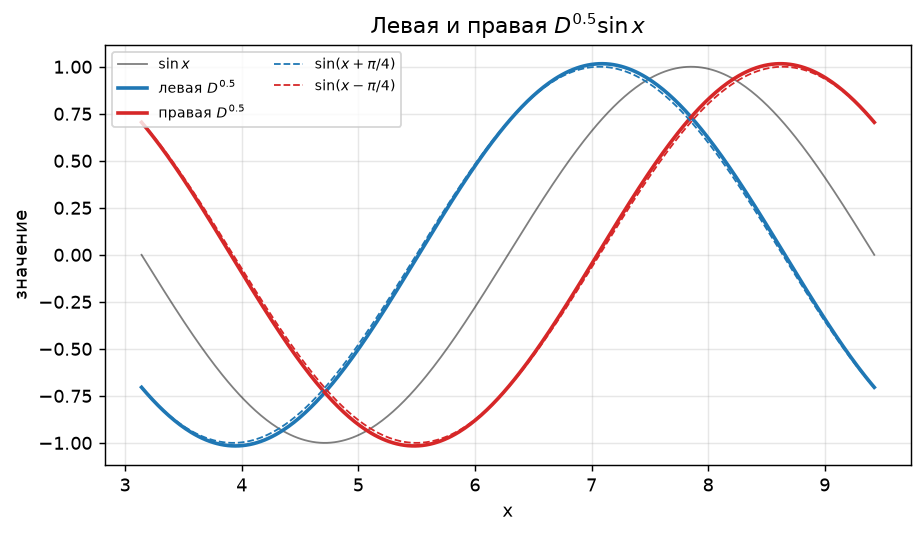
\includegraphics[width=0.85\textwidth]{left_vs_right.png}
\caption{Левая и правая $\D^{0{,}5}\sin x$ со сдвигом фазы в разные стороны, $\sin(x\pm\pi/4)$ ($h=0{,}01$, $N=500$)}
\label{fig:lr}
\end{figure}

У $\tan x$ есть разрыв в $\pi/2$, и около него значения растут неограниченно (рисунок~\ref{fig:tan}). Уже на отрезке от $0{,}2$ до $1{,}3$ и функция, и её дробная производная резко уходят вверх к правому краю. Метод формально работает, но интервал держат в стороне от особой точки. Устойчивость, как видно, упирается не только в параметры схемы, но и в саму функцию.

\begin{figure}[htbp]
\centering
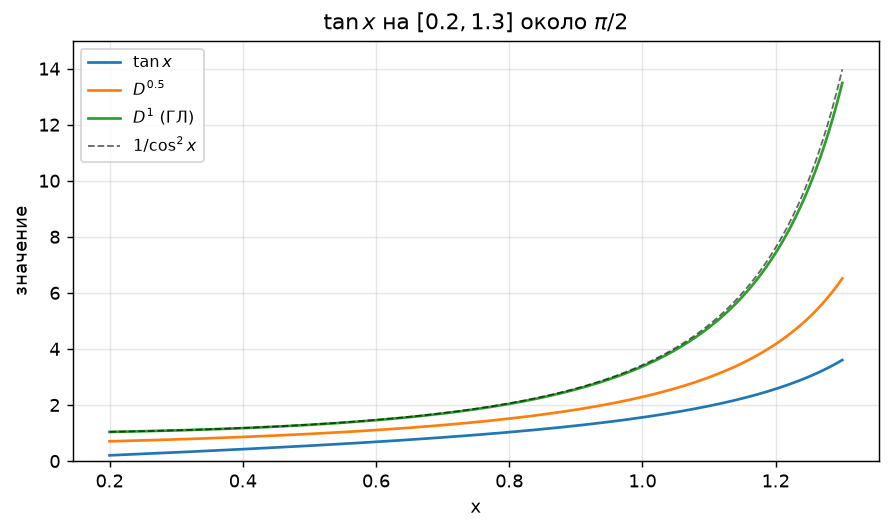
\includegraphics[width=0.8\textwidth]{tan_instability.png}
\caption{Поведение $\tan x$ и его дробной производной вблизи разрыва в точке $\pi/2$ ($h=0{,}01$, $N=100$, память $L=1$)}
\label{fig:tan}
\end{figure}

\subsection{Карта дробных производных}

Если построить $\D^{\alpha}\sin x$ для непрерывной сетки порядков, получается сводная карта значений (рисунок~\ref{fig:atlas}). По горизонтали отложен $x$, по вертикали порядок $\alpha$ от $0$ до $2$, цветом показано значение производной. Максимумы и минимумы идут наклонными полосами. При росте $\alpha$ картина равномерно сдвигается влево, и сдвиг линеен по $\alpha$.

\begin{figure}[htbp]
\centering
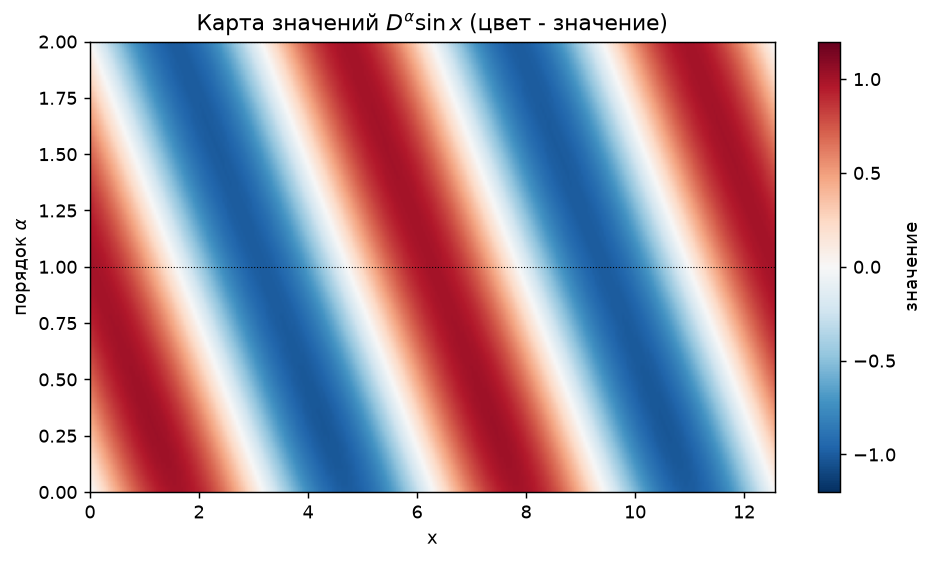
\includegraphics[width=0.9\textwidth]{atlas.png}
\caption{Карта значений $\D^{\alpha}\sin x$ на плоскости $(x,\alpha)$, цвет соответствует значению производной ($h=0{,}01$, $N=500$)}
\label{fig:atlas}
\end{figure}

\section{Точность, устойчивость и пути её повышения}

В этой главе метод рассматривается со стороны самих чисел. Речь о том, какие свойства коэффициентов поддаются проверке и где у точности есть предел, который частично удаётся обойти.

\subsection{Аналитическая оценка порядка аппроксимации}
\label{sec:order}

Первый порядок $O(h)$ из таблиц сходимости (раздел~\ref{sec:conv}) можно получить и аналитически, не только численно. Производящая функция коэффициентов равна
\begin{equation}
\sum_{k=0}^{\infty}c_k^{(\alpha)}z^k=\sum_{k=0}^{\infty}(-1)^k\binom{\alpha}{k}z^k=(1-z)^{\alpha}.
\end{equation}
Применим разностный оператор $\delta_h^{\alpha}f(x)=\sum_{k\geqslant0}c_k^{(\alpha)}f(x-kh)$ к гармонике $f(x)=e^{i\omega x}$. Поскольку $f(x-kh)=e^{i\omega x}e^{-i\omega kh}$, сумма сворачивается в производящую функцию при $z=e^{-i\omega h}$:
\begin{equation}
\delta_h^{\alpha}e^{i\omega x}=(1-e^{-i\omega h})^{\alpha}e^{i\omega x},\qquad
\D^{\alpha}_{h}e^{i\omega x}=\left(\frac{1-e^{-i\omega h}}{h}\right)^{\alpha}e^{i\omega x}.
\end{equation}
Из разложения $1-e^{-i\omega h}=i\omega h\,\bigl(1-\tfrac{i\omega h}{2}+O(h^2)\bigr)$ следует
\begin{equation}
\left(\frac{1-e^{-i\omega h}}{h}\right)^{\alpha}=(i\omega)^{\alpha}\left(1-\frac{\alpha}{2}\,i\omega h+O(h^2)\right)=(i\omega)^{\alpha}-\frac{\alpha}{2}(i\omega)^{\alpha+1}h+O(h^2).
\end{equation}
Множитель $(i\omega)^{\alpha}$ задаёт символ точной производной $\D^{\alpha}$, а $(i\omega)^{\alpha+1}$ отвечает $\D^{\alpha+1}$ (при нецелом $\alpha$ берётся главная ветвь степенной функции, $i^{\alpha}=e^{i\pi\alpha/2}$, что отвечает левому оператору в форме Лиувилля и согласуется с фазовым сдвигом~\eqref{eq:trig}). Поэтому для гладкой функции
\begin{equation}
\D^{\alpha}_{h}f(x)=\D^{\alpha}f(x)-\frac{\alpha}{2}\,h\,\D^{\alpha+1}f(x)+O(h^2).
\label{eq:order}
\end{equation}
Отсюда сразу виден первый порядок $O(h)$, причём ведущая ошибка пропорциональна $\D^{\alpha+1}f$. При $\alpha=1$ это $-\tfrac{h}{2}f''$, и для $\sin x$ в точке $x=1$ по модулю получается $\tfrac{h}{2}|\!\sin1|\approx0{,}42\,h$. Таблица~\ref{tab:conv} это и показывает. При $h=0{,}1$ ошибка $0{,}041\approx0{,}42\cdot0{,}1$. Разложение~\eqref{eq:order} объясняет и экстраполяцию Ричардсона. Она построена так, чтобы погасить именно линейный по $h$ член.

У этой оценки есть важная оговорка. Разложение~\eqref{eq:order} получено для полной суммы с бесконечной историей, то есть в нём учтена только ошибка дискретизации. При конечном $N$ к ней добавляется ошибка усечения, которую символьный анализ не видит. Дальние коэффициенты $|c_k|\sim k^{-(\alpha+1)}$ отбрасываются, и их вклад убывает как $N^{-\alpha}$ (раздел~\ref{sec:N}). Полная погрешность складывается из двух независимых частей, дискретизации $O(h)$ и усечения $O(N^{-\alpha})$. В режиме нижнего предела $a=0$ степенная история обрывается естественно при $N=\lfloor x/h\rfloor$, член усечения исчезает, и остаётся чистый $O(h)$; в режиме конечной памяти $L=Nh$ заметны оба слагаемых, и уменьшать одно только $h$ при коротком $N$ бесполезно.

\subsection{Проверка через сумму коэффициентов}

У коэффициентов есть свойство, не зависящее ни от функции, ни от точки. Сумма всех коэффициентов равна
\begin{equation}
\sum_{k=0}^{\infty}c_k^{(\alpha)}=\sum_{k=0}^{\infty}(-1)^k\binom{\alpha}{k}=(1-1)^{\alpha}=0\quad(\alpha>0).
\end{equation}
Тогда частичные суммы $S_n=\sum_{k=0}^{n}c_k$ обязаны стремиться к нулю (таблица~\ref{tab:sums}). Они убывают к нулю медленно. Для $\alpha=0{,}5$ при $n=10$ сумма ещё $0{,}176$, при $n=100$ уже $0{,}056$, а при $n=500$ всего $0{,}025$. Это согласуется с медленным затуханием коэффициентов и служит независимым тестом, ведь при ошибке в рекуррентной формуле суммы не стремились бы к нулю.

\begin{table}[htbp]
\centering
\caption{Частичные суммы коэффициентов $S_n=\sum_{k=0}^{n}c_k$ (стремятся к нулю при $\alpha>0$)}
\label{tab:sums}
\begin{tabular}{|r|r|r|r|}
\hline
$n$ & $\alpha=0{,}25$ & $\alpha=0{,}5$ & $\alpha=0{,}75$ \\
\hline
$1$   & $0{,}750$ & $0{,}500$ & $0{,}250$ \\
\hline
$5$   & $0{,}536$ & $0{,}246$ & $0{,}081$ \\
\hline
$10$  & $0{,}455$ & $0{,}176$ & $0{,}049$ \\
\hline
$50$  & $0{,}306$ & $0{,}080$ & $0{,}015$ \\
\hline
$100$ & $0{,}258$ & $0{,}056$ & $0{,}009$ \\
\hline
$500$ & $0{,}173$ & $0{,}025$ & $0{,}003$ \\
\hline
\end{tabular}
\end{table}

\subsection{Порядок усечения по числу членов}

На лог-лог графике (рисунок~\ref{fig:Ntr}) ошибка усечения против $N$ ложится почти на прямую, наклон растёт от примерно $0{,}8$ при малых $N$ до примерно $1{,}3$ при больших. Это быстрее, чем даёт теоретическая оценка короткой памяти $N^{-\alpha}=N^{-0{,}5}$ (пунктир на графике): для $\sin x$ помогает то, что значения ограничены и знакопеременны, и дальние слагаемые частично гасят друг друга.

\begin{figure}[htbp]
\centering
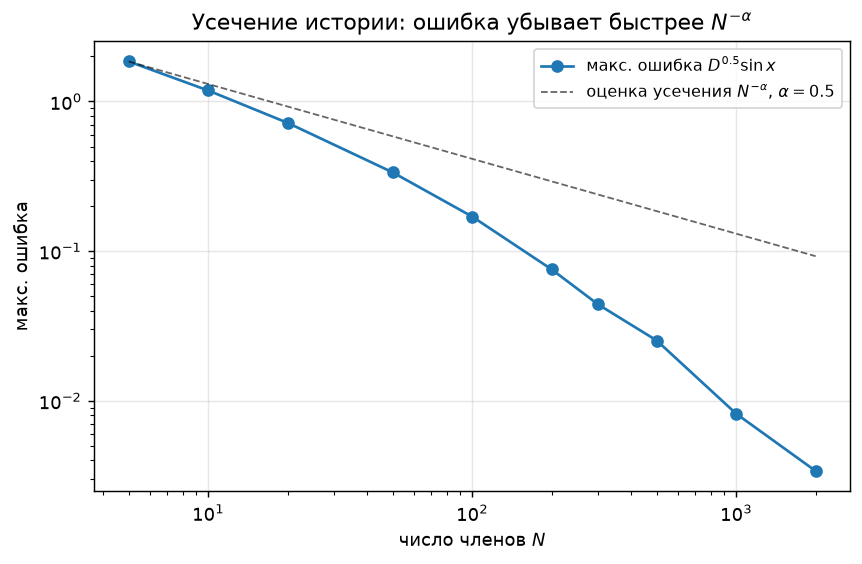
\includegraphics[width=0.8\textwidth]{N_truncation.png}
\caption{Ошибка усечения $\D^{0{,}5}\sin x$ в зависимости от числа членов $N$ в лог-лог осях ($h=0{,}01$)}
\label{fig:Ntr}
\end{figure}

\subsection{Предел точности и порог округления}
\label{sec:floor}

Уменьшать шаг бесконечно нельзя. Деление на $h^{\alpha}$ усиливает ошибки округления. Для $\D^1\sin x$ в точке $x=1$ шаг $h$ менялся от $0{,}1$ до $10^{-11}$ (таблица~\ref{tab:floor}, рисунок~\ref{fig:floor}).

\begin{table}[htbp]
\centering
\caption{Ошибка $\D^1\sin x$ в точке $x=1$ при уменьшении шага $h$}
\label{tab:floor}
\begin{tabular}{|r|r|}
\hline
$h$ & Ошибка \\
\hline
$10^{-1}$ & $4{,}1\cdot10^{-2}$ \\
\hline
$10^{-3}$ & $4{,}2\cdot10^{-4}$ \\
\hline
$10^{-5}$ & $4{,}2\cdot10^{-6}$ \\
\hline
$10^{-7}$ & $4{,}1\cdot10^{-8}$ \\
\hline
$10^{-8}$ & $8{,}1\cdot10^{-9}$ \\
\hline
$10^{-9}$ & $5{,}8\cdot10^{-8}$ \\
\hline
$10^{-11}$& $1{,}2\cdot10^{-6}$ \\
\hline
\end{tabular}
\end{table}

Сначала ошибка падает пропорционально $h$. Около $h\approx10^{-8}$ она достигает минимума примерно $8\cdot10^{-9}$, дальше снова растёт. При $h=10^{-11}$ ошибка уже $1{,}2\cdot10^{-6}$. Слева работает дискретизация ($\sim h/2$), справа округление ($\sim\varepsilon/h$, где $\varepsilon$ обозначает машинную точность), а минимум стоит около $h\sim\sqrt{\varepsilon}\approx10^{-8}$. Базовый $h=0{,}01$ находится далеко в безопасной зоне.

\begin{figure}[htbp]
\centering
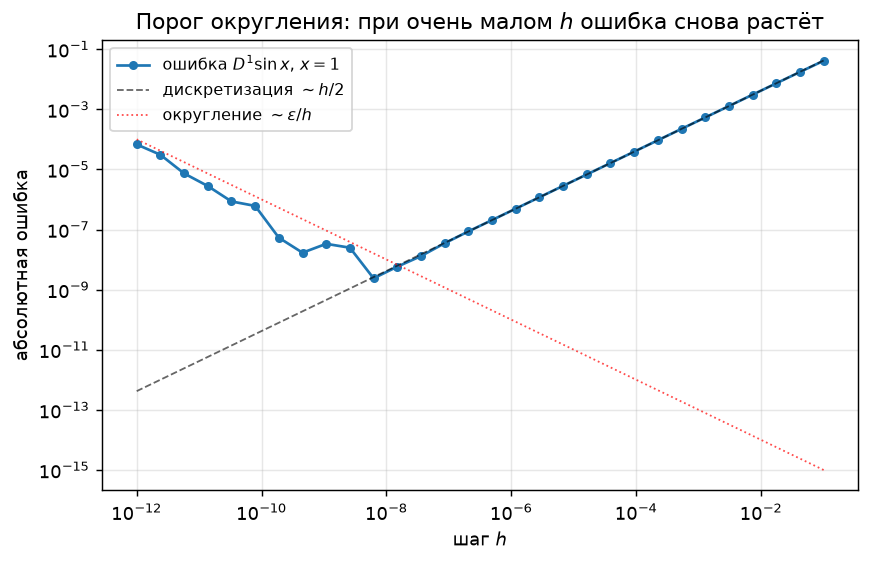
\includegraphics[width=0.8\textwidth]{rounding_floor.png}
\caption{Порог округления ошибки $\D^1\sin x$ в точке $x=1$}
\label{fig:floor}
\end{figure}

\subsection{Повышение порядка через экстраполяцию Ричардсона}

Раз ошибка ведёт себя как $C\,h+O(h^2)$, линейный член можно погасить. Комбинация результатов на шагах $h$ и $h/2$
\begin{equation}
R(h)=2\,\D^{\alpha}_{h/2}f(x)-\D^{\alpha}_{h}f(x)
\end{equation}
убирает слагаемое $C\,h$ и оставляет $O(h^2)$ \cite{podlubny}. Проверка проведена на $\D^1\sin x$ в точке $x=1$ (таблица~\ref{tab:rich}) и на дробном порядке $\D^{0{,}5}x^2$ в точке $x=2$ (таблица~\ref{tab:richfrac}).

\begin{table}[htbp]
\centering
\caption{Обычная схема против экстраполяции Ричардсона для $\D^1\sin x$, $x=1$}
\label{tab:rich}
\begin{tabular}{|r|r|r|r|r|}
\hline
$h$ & Ошибка обычн. & Отнош. & Ошибка Ричардсон & Отнош. \\
\hline
$0{,}200$  & $0{,}0803$ & ---     & $0{,}00200$  & --- \\
\hline
$0{,}100$  & $0{,}0411$ & $1{,}95$& $0{,}00048$  & $4{,}21$ \\
\hline
$0{,}050$  & $0{,}0208$ & $1{,}98$& $0{,}00012$  & $4{,}11$ \\
\hline
$0{,}025$  & $0{,}0105$ & $1{,}99$& $0{,}000029$ & $4{,}06$ \\
\hline
$0{,}0125$ & $0{,}0052$ & $1{,}99$& $0{,}0000072$& $4{,}03$ \\
\hline
$0{,}00625$& $0{,}0026$ & $2{,}00$& $0{,}0000018$& $4{,}01$ \\
\hline
\end{tabular}
\end{table}

\begin{table}[htbp]
\centering
\caption{Экстраполяция Ричардсона для дробного порядка $\D^{0{,}5}x^2$, $x=2$ (режим $a=0$)}
\label{tab:richfrac}
\begin{tabular}{|r|r|r|r|}
\hline
$h$ & Ошибка обычн. & Ошибка Ричардсон & Отнош. Ричардсона \\
\hline
$0{,}040$  & $0{,}0319$ & $3{,}3\cdot10^{-5}$ & --- \\
\hline
$0{,}020$  & $0{,}0159$ & $8{,}3\cdot10^{-6}$ & $4{,}00$ \\
\hline
$0{,}010$  & $0{,}0080$ & $2{,}1\cdot10^{-6}$ & $4{,}00$ \\
\hline
$0{,}005$  & $0{,}0040$ & $5{,}2\cdot10^{-7}$ & $4{,}00$ \\
\hline
\end{tabular}
\end{table}

У обычной схемы при уменьшении $h$ вдвое ошибка падает в $2$ раза (первый порядок), у экстраполяции в $4$ раза (второй порядок, $O(h^2)$). При $\alpha=1$ уже при $h=0{,}2$ экстраполяция даёт ошибку $0{,}002$ против $0{,}08$ у обычной схемы. Платой за это становится второй расчёт с половинным шагом. Для дробного порядка $\alpha=0{,}5$ отношение тоже близко к $4$ (таблица~\ref{tab:richfrac}). Рисунки~\ref{fig:rich} и~\ref{fig:richfrac} показывают это в лог-лог осях.

\begin{figure}[htbp]
\centering
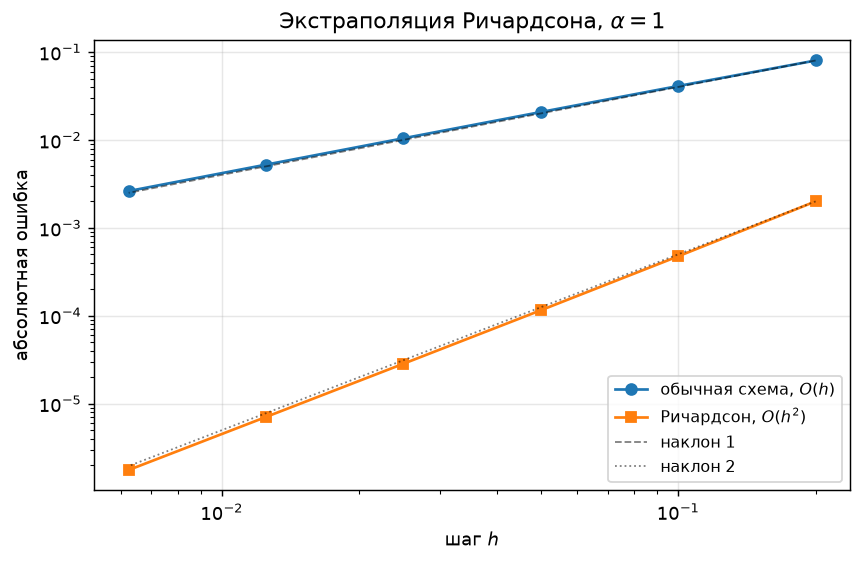
\includegraphics[width=0.78\textwidth]{richardson.png}
\caption{Экстраполяция Ричардсона против обычной схемы для $\D^1\sin x$}
\label{fig:rich}
\end{figure}

\begin{figure}[htbp]
\centering
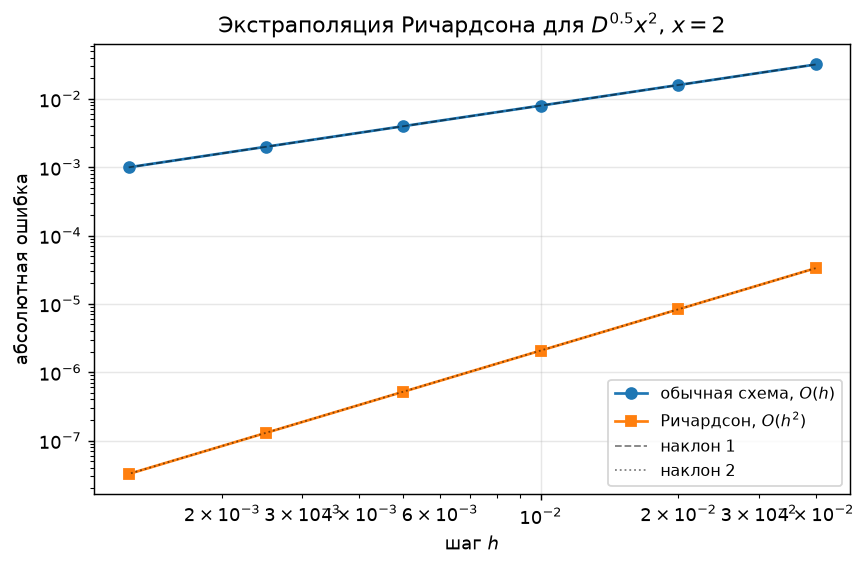
\includegraphics[width=0.78\textwidth]{richardson_frac.png}
\caption{Экстраполяция Ричардсона для $\D^{0{,}5}x^2$ в режиме $a=0$}
\label{fig:richfrac}
\end{figure}

\subsection{Нижний предел против конечной памяти}
\label{sec:regime-exp}

Покажем численно, что режимы из раздела~\ref{sec:regimes} дают разные значения. Возьмём $\D^{0{,}5}x^2$ в точке $x=2$, $h=0{,}01$ и посчитаем тремя способами (таблица~\ref{tab:regimecmp}). Точное значение в режиме $a=0$ равно $\Gamma(3)/\Gamma(2{,}5)\cdot 2^{1{,}5}\approx4{,}255$.

\begin{table}[htbp]
\centering
\caption{Один и тот же $\D^{0{,}5}x^2$ в точке $x=2$ при разных режимах, $h=0{,}01$}
\label{tab:regimecmp}
\begin{tabular}{|l|r|r|r|}
\hline
Режим & $N$ & Значение & Эталон $a=0$ \\
\hline
Нижний предел $a=0$. & $200$ & $4{,}247$ & $4{,}255$ \\
\hline
Конечная память $L=5$. & $500$ & $3{,}944$ & --- \\
\hline
Фиксированное $N=50$. & $50$  & $4{,}706$ & --- \\
\hline
\end{tabular}
\end{table}

Три режима дают $4{,}247$, $3{,}944$ и $4{,}706$, то есть расходятся на десятки процентов. С гамма-формулой совпадает только режим $a=0$ (отклонение $0{,}008$, порядка $h$). Режимы конечной памяти считают дробную производную с обрезанной историей, и гамма-формула для них уже не эталон. Поэтому у каждой таблицы в подписи указан свой режим.

\subsection{Совместное влияние шага и числа членов}

Рисунок~\ref{fig:heat} показывает совместное влияние $h$ и $N$ для целого порядка. Цветом отмечен десятичный логарифм максимальной ошибки $\D^1\sin x$. Для $\alpha=1$ ошибка определяется почти только шагом $h$ (горизонтальные полосы), потому что коэффициенты обрываются и $N$ роли не играет.

\begin{figure}[htbp]
\centering
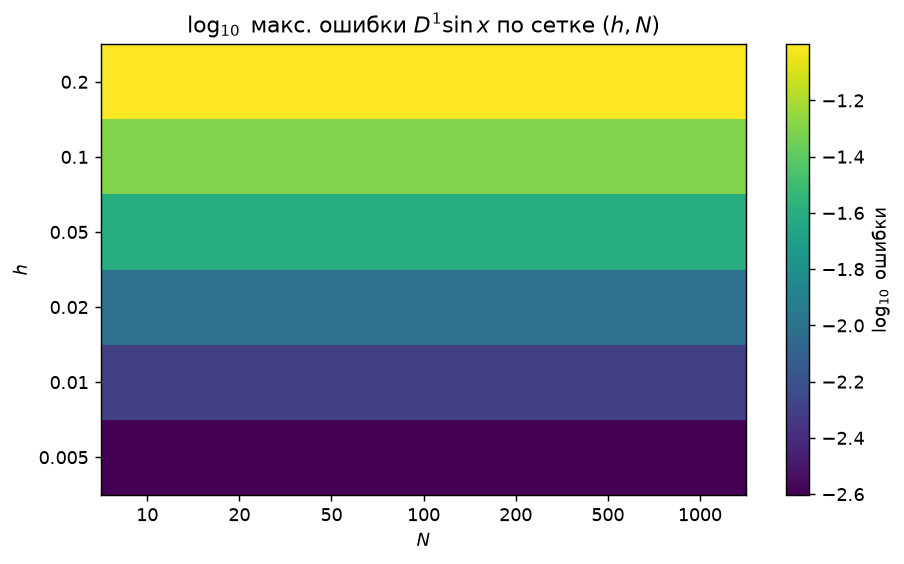
\includegraphics[width=0.85\textwidth]{error_heatmap.png}
\caption{Карта максимальной ошибки $\D^1\sin x$ по сетке $(h, N)$}
\label{fig:heat}
\end{figure}

Для дробного порядка картина другая (рисунок~\ref{fig:heatfrac}). Полосы наклонные, ошибка $\D^{0{,}5}\sin x$ падает и при уменьшении $h$, и при росте $N$. Минимум достигается в правом нижнем углу, где одновременно мелкий шаг и длинная история.

\begin{figure}[htbp]
\centering
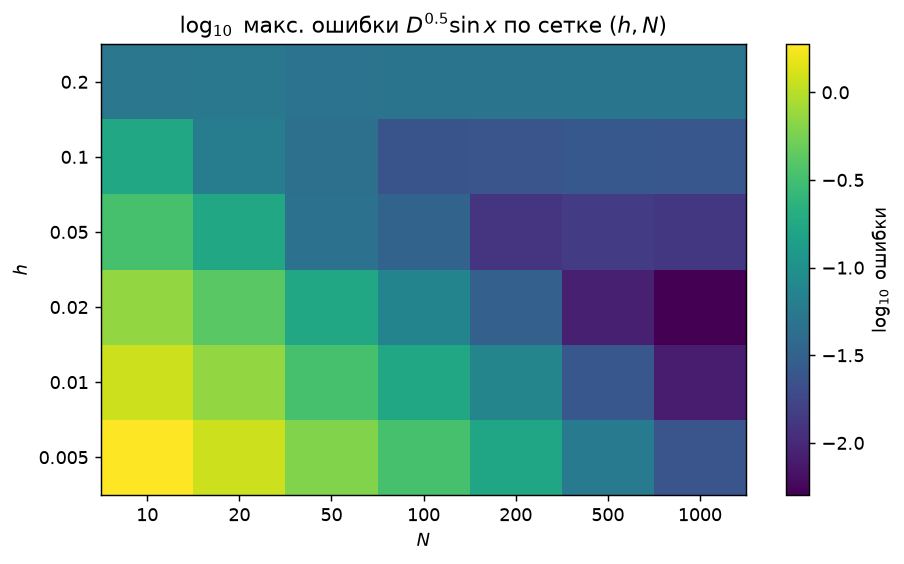
\includegraphics[width=0.85\textwidth]{error_heatmap_frac.png}
\caption{Карта максимальной ошибки $\D^{0{,}5}\sin x$ по сетке $(h, N)$}
\label{fig:heatfrac}
\end{figure}

\subsection{Сдвинутая схема Грюнвальда}
\label{sec:shifted}

В стандартной схеме самый правый узел суммы совпадает с самой точкой $x$ (сдвиг $p=0$). Сдвинутая схема Грюнвальда берёт узлы $x-(k-p)h$, сдвигая шаблон на $p$ шагов вправо \cite{meerschaert}:
\begin{equation}
\D^{\alpha,p}_{h}f(x)=\frac{1}{h^{\alpha}}\sum_{k=0}^{N}c_k^{(\alpha)}f\bigl(x-(k-p)h\bigr).
\end{equation}
Коэффициенты те же, меняется только положение узлов, и при целом сдвиге $p=1$ верхний узел равен $x+h$. Такая схема тоже имеет первый порядок $O(h)$, но её ценность в другом. При дискретизации уравнений с дробной производной по пространству именно сдвиг $p=1$ делает разностную матрицу устойчивой, тогда как несдвинутая схема ($p=0$) даёт неустойчивую дискретизацию \cite{meerschaert}.

На отдельном значении производной сдвиг почти незаметен, зато при дискретизации уравнений становится принципиальным. Аномальная диффузия, упомянутая во введении, описывается уравнением с дробной производной по пространству, $\partial_t u=K\,\D^{\beta}_{x}u$ при $1<\beta<2$. Если оператор $\D^{\beta}_{x}$ заменить обычной суммой Грюнвальда--Летникова ($p=0$), собственные значения разностной матрицы получают положительную вещественную часть, и явная схема по времени расходится. Сдвиг на один узел ($p=1$) делает эти вещественные части неположительными и возвращает устойчивость \cite{meerschaert}. Так малозаметный на одной точке параметр $p$ определяет устойчивость всей схемы, и ради этого сдвинутый вариант включён в работу рядом со стандартным.

Сравнение на $\D^{0{,}5}x^2$ в точке $x=2$ (режим $a=0$, эталон $\approx4{,}255$) приведено в таблице~\ref{tab:shifted}. Обе схемы сходятся с первым порядком, отношение ошибок близко к $2$. При одном и том же $h$ сдвинутая схема даёт примерно втрое большую ошибку, и это плата за сдвиг шаблона. В лог-лог осях обе зависимости ложатся в прямые с наклоном $1$ (рисунок~\ref{fig:shifted}).

\begin{table}[htbp]
\centering
\caption{Стандартная и сдвинутая схемы Грюнвальда для $\D^{0{,}5}x^2$, $x=2$ (режим $a=0$)}
\label{tab:shifted}
\begin{tabular}{|r|r|r|r|r|}
\hline
$h$ & Ошибка ГЛ ($p=0$) & Отнош. & Ошибка сдвиг ($p=1$) & Отнош. \\
\hline
$0{,}0400$ & $0{,}0318$  & ---     & $0{,}0961$  & --- \\
\hline
$0{,}0200$ & $0{,}0159$  & $2{,}00$& $0{,}0480$  & $2{,}00$ \\
\hline
$0{,}0100$ & $0{,}0080$  & $2{,}00$& $0{,}0240$  & $2{,}00$ \\
\hline
$0{,}0050$ & $0{,}0040$  & $2{,}00$& $0{,}0120$  & $2{,}00$ \\
\hline
$0{,}0025$ & $0{,}0020$  & $2{,}00$& $0{,}0060$  & $2{,}00$ \\
\hline
\end{tabular}
\end{table}

\begin{figure}[htbp]
\centering
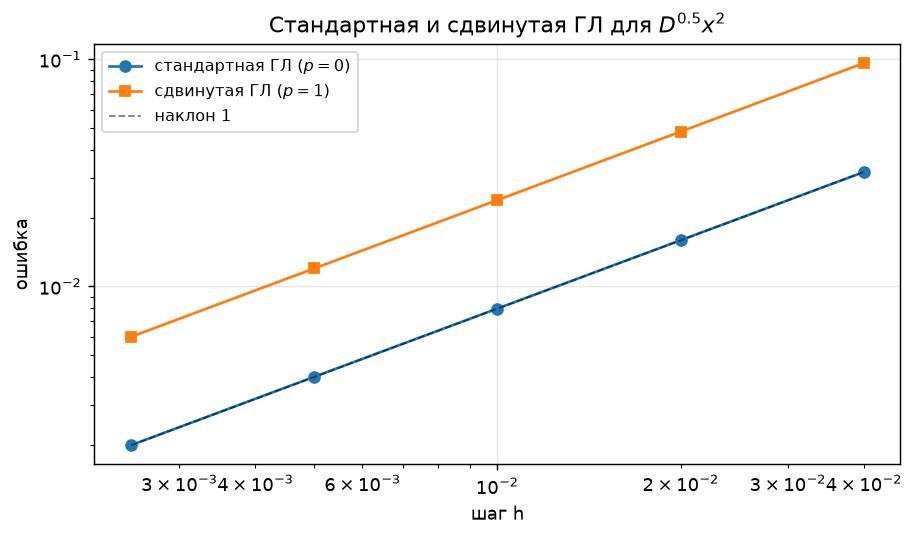
\includegraphics[width=0.78\textwidth]{shifted_convergence.png}
\caption{Сходимость стандартной и сдвинутой схем Грюнвальда для $\D^{0{,}5}x^2$}
\label{fig:shifted}
\end{figure}

\subsection{Сравнение с производной Капуто}
\label{sec:caputo}

Определение Капуто, введённое в главе~1, на практике считают по схеме L1. Для $0<\alpha<1$ и нижнего предела $0$
\begin{equation}
\D^{\alpha}_{C}f(t_n)\approx\frac{1}{\Gamma(2-\alpha)\,h^{\alpha}}\sum_{k=0}^{n-1}b_k\bigl(f(t_{n-k})-f(t_{n-k-1})\bigr),\qquad b_k=(k+1)^{1-\alpha}-k^{1-\alpha},
\end{equation}
где $t_j=jh$. В отличие от Грюнвальда--Летникова, схема L1 опирается не на сами значения функции, а на её приращения. Поэтому производная постоянной по Капуто равна нулю, тогда как у Грюнвальда--Летникова и Римана--Лиувилля $\D^{\alpha}1=x^{-\alpha}/\Gamma(1-\alpha)\neq0$. На гладких функциях схема L1 имеет порядок аппроксимации $O(h^{2-\alpha})$ \cite{diethelm}, то есть при $0<\alpha<1$ точнее первого порядка $O(h)$ стандартной схемы Грюнвальда--Летникова. В работе она привлекается лишь для иллюстрации граничного слагаемого, отличающего Капуто от Римана--Лиувилля.

Определения связаны соотношением $\D^{\alpha}_{RL}f=\D^{\alpha}_{C}f+f(0)\,x^{-\alpha}/\Gamma(1-\alpha)$. Численное сравнение на $e^x$ при $\alpha=0{,}5$, $h=0{,}005$ (таблица~\ref{tab:caputo}) его подтверждает. Разность Грюнвальда--Летникова и Капуто близка к слагаемому $f(0)\,x^{-\alpha}/\Gamma(1-\alpha)$ с $f(0)=1$. С ростом $x$ это слагаемое убывает как $x^{-\alpha}$, и определения сближаются (рисунок~\ref{fig:caputo}). Для функций с $f(0)=0$, например $x^2$, обе схемы совпадают с формулой через гамма-функцию.

\begin{table}[htbp]
\centering
\caption{Грюнвальд--Летников и Капуто для $\D^{0{,}5}e^x$, $h=0{,}005$}
\label{tab:caputo}
\begin{tabular}{|r|r|r|r|r|}
\hline
$x$ & ГЛ ($a=0$) & Капуто (L1) & ГЛ $-$ Капуто & $f(0)x^{-\alpha}/\Gamma(1-\alpha)$ \\
\hline
$0{,}5$ & $1{,}920$  & $1{,}125$  & $0{,}795$ & $0{,}798$ \\
\hline
$0{,}9$ & $2{,}609$  & $2{,}017$  & $0{,}591$ & $0{,}595$ \\
\hline
$1{,}3$ & $3{,}767$  & $3{,}277$  & $0{,}490$ & $0{,}495$ \\
\hline
$1{,}7$ & $5{,}543$  & $5{,}117$  & $0{,}426$ & $0{,}433$ \\
\hline
$2{,}1$ & $8{,}215$  & $7{,}835$  & $0{,}380$ & $0{,}389$ \\
\hline
$2{,}5$ & $12{,}215$ & $11{,}873$ & $0{,}342$ & $0{,}357$ \\
\hline
\end{tabular}
\end{table}

\begin{figure}[htbp]
\centering
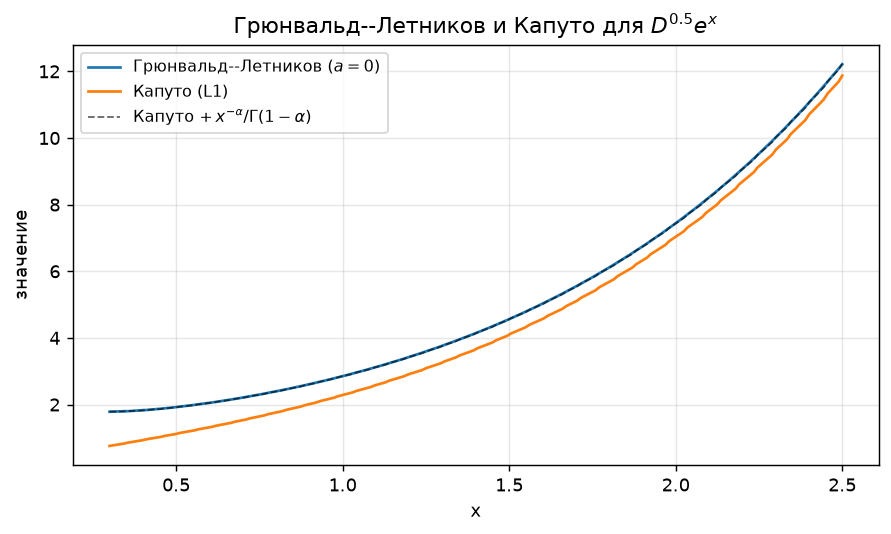
\includegraphics[width=0.8\textwidth]{gl_vs_caputo.png}
\caption{Грюнвальд--Летников и Капуто для $\D^{0{,}5}e^x$ ($h=0{,}005$); пунктиром показана сумма Капуто и граничной поправки}
\label{fig:caputo}
\end{figure}

\FloatBarrier
\clearpage

\phantomsection
\addcontentsline{toc}{section}{Заключение}
\section*{Заключение}

Главным результатом работы стала сводная таблица дробных производных элементарных функций (таблица~\ref{tab:master}), построенная численным методом Грюнвальда--Летникова и сверенная с замкнутыми формами из справочной таблицы~\ref{tab:reftable}. Чтобы её получить, реализовано вычисление дробных производных по формуле Грюнвальда--Летникова и собран небольшой программный комплекс. В него входят модуль расчёта, набор функций, генерация таблиц и графиков, командный запуск, автоматические тесты и веб-интерфейс на React с интерактивным графиком Plotly. Метод хорошо ложится на табличные вычисления, поскольку записывается рекуррентной формулой для коэффициентов и одним матричным умножением для суммы по сетке.

Результаты подтверждены численно. На целых порядках реализация прошла проверку. $\D^1\sin x$ приближает $\cos x$ с ошибкой порядка $h$, $\D^2 x^2$ даёт ровно $2$, а для $x^2$ при $\alpha=1$ ошибка равна ровно $h$ из-за смещения левой разности.

Сходимость по шагу имеет первый порядок. При уменьшении $h$ вдвое ошибка падает вдвое, одинаково для целого ($\sin x$) и дробного ($x^2$, $\alpha=0{,}5$) порядка. В режиме нижнего предела $a=0$ дробная производная $x^2$ согласуется с аналитической формулой через гамма-функцию с ошибкой порядка $h$. Режимы конечной памяти дают другие значения, и сравнивать их с гамма-формулой уже нельзя.

Параметры $h$ и $N$ влияют по-разному. Шаг $h$ задаёт точность сетки. Ошибка $\D^1\sin x$ менялась от $0{,}05$ при $h=0{,}1$ до $0{,}0005$ при $h=0{,}001$. Число $N$ задаёт длину памяти. Для $\D^{0{,}5}\sin x$ при $N=5$ ошибка была $1{,}85$, а при $N=1000$ упала до $0{,}008$. Причина заключается в медленном затухании коэффициентов $|c_k|\sim k^{-(\alpha+1)}$.

Углублённый разбор точности дал ещё несколько выводов. Проверка через сумму коэффициентов ($\sum c_k=0$) подтвердила корректность рекуррентной формулы. У ошибки есть порог около $h\sim10^{-8}$ (минимум $\approx8\cdot10^{-9}$), ниже которого округление при делении на $h^{\alpha}$ её увеличивает. Экстраполяция Ричардсона поднимает порядок точности до $O(h^2)$ как для целого, так и для дробного порядка. Сравнение левой и правой схем показало, что для дробного порядка это два разных результата со сдвигом фазы в противоположные стороны.

Первый порядок $O(h)$ получен не только численно, но и аналитически. Разложение символа схемы даёт $\D^{\alpha}_h f=\D^{\alpha}f-\tfrac{\alpha}{2}h\,\D^{\alpha+1}f+O(h^2)$, и это же разложение объясняет работу экстраполяции Ричардсона. Сдвинутая схема Грюнвальда ($p=1$) сохраняет порядок $O(h)$, но даёт устойчивую дискретизацию для уравнений с дробной производной. Численное сравнение с производной Капуто подтвердило граничное соотношение $\D^{\alpha}_{RL}f=\D^{\alpha}_{C}f+f(0)x^{-\alpha}/\Gamma(1-\alpha)$. Определения различаются на слагаемое, убывающее как $x^{-\alpha}$, а производная постоянной по Капуто равна нулю.

Есть у метода и ограничения, и о них честнее сказать прямо. Он даёт численное приближение всего первого порядка, и результат заметно зависит от шага, длины истории и поведения самой функции. На гладких функциях ($\sin x$, $\cos x$, $e^x$) он ведёт себя устойчиво. Зато для $e^x$ абсолютная ошибка растёт вместе со значением функции, для $\ln x$ приходится следить за условием $x-Nh>0$, а для $\tan x$ интервал вообще держим подальше от разрыва. Уверенность в правильности складывается из нескольких независимых проверок. Это совпадение на целых порядках, нулевая сумма коэффициентов и сверка с аналитическими формулами. По строгости это инженерная проверка, и доказательства она не заменяет.

Возможные направления развития включают схемы второго порядка (взвешенные сдвинутые формулы), решение дробных дифференциальных уравнений на основе полученной дискретизации, автоматический подбор $N$ по заданной точности и ускорение расчёта на равномерной сетке через свёртку.

\clearpage
\begingroup
\raggedright
\begin{thebibliography}{15}
\phantomsection
\addcontentsline{toc}{section}{Список литературы}
\bibitem{samko} Самко, С. Г. Интегралы и производные дробного порядка и некоторые их приложения / С.~Г.~Самко, А.~А.~Килбас, О.~И.~Маричев. --- Минск : Наука и техника, 1987. --- 688~с.
\bibitem{diethelm} Diethelm, K. The Analysis of Fractional Differential Equations / K.~Diethelm. --- Berlin : Springer, 2010. --- 247~p.
\bibitem{dfff} Diethelm, K. Algorithms for the fractional calculus: a selection of numerical methods / K.~Diethelm, N.~J.~Ford, A.~D.~Freed, Yu.~Luchko // Computer Methods in Applied Mechanics and Engineering. --- 2005. --- Vol.~194, № 6--8. --- P.~743--773.
\bibitem{harris} Harris, C. R. Array programming with NumPy / C.~R.~Harris, K.~J.~Millman, S.~J.~van der Walt [et al.] // Nature. --- 2020. --- Vol.~585. --- P.~357--362.
\bibitem{hunter} Hunter, J. D. Matplotlib: a 2D graphics environment / J.~D.~Hunter // Computing in Science \& Engineering. --- 2007. --- Vol.~9, № 3. --- P.~90--95.
\bibitem{lubich} Lubich, C. Discretized fractional calculus / C.~Lubich // SIAM Journal on Mathematical Analysis. --- 1986. --- Vol.~17, № 3. --- P.~704--719.
\bibitem{meerschaert} Meerschaert, M. M. Finite difference approximations for fractional advection-dispersion flow equations / M.~M.~Meerschaert, C.~Tadjeran // Journal of Computational and Applied Mathematics. --- 2004. --- Vol.~172, № 1. --- P.~65--77.
\bibitem{oldham} Oldham, K. B. The Fractional Calculus: Theory and Applications of Differentiation and Integration to Arbitrary Order / K.~B.~Oldham, J.~Spanier. --- New York : Academic Press, 1974. --- 234~p.
\bibitem{podlubny} Podlubny, I. Fractional Differential Equations / I.~Podlubny. --- San Diego : Academic Press, 1999. --- 340~p.
\bibitem{numpydoc} NumPy documentation [Электронный ресурс]. --- URL: https://numpy.org/doc/
\bibitem{pydoc} Python documentation [Электронный ресурс]. --- URL: https://docs.python.org/3/
\bibitem{reactdoc} React documentation [Электронный ресурс]. --- URL: https://react.dev/
\bibitem{vitedoc} Vite documentation [Электронный ресурс]. --- URL: https://vite.dev/
\bibitem{plotlydoc} Plotly.js documentation [Электронный ресурс]. --- URL: https://plotly.com/javascript/
\bibitem{bundoc} Bun documentation [Электронный ресурс]. --- URL: https://bun.sh/docs
\end{thebibliography}
\endgroup

\clearpage
\appendix
\addtocontents{toc}{\protect\let\protect\numberline\protect\appnumberline}
\renewcommand{\thesection}{Приложение~\Asbuk{section}}
\renewcommand{\thesubsection}{\Asbuk{section}.\arabic{subsection}}
\section{Структура проекта и запуск}

Назначение модулей описано в таблице~\ref{tab:struct}. Дерево каталога:

\begin{lstlisting}
CourseWork/
|-- fractional.py
|-- functions.py
|-- experiments.py
|-- tables.py
|-- plots.py
|-- main.py
|-- requirements.txt
|-- README.md
|-- web/
|   |-- package.json
|   |-- src/
|   |   |-- domain/
|   |   |-- hooks/
|   |   +-- components/
|-- tests/
|   |-- conftest.py
|   |-- test_coefficients.py
|   |-- test_fractional_orders.py
|   |-- test_function_domains.py
|   |-- test_integer_orders.py
|   |-- test_alt_schemes.py
|   +-- test_master_table.py
|-- graphs/
|-- tables/
+-- report/
\end{lstlisting}

Зависимости Python перечислены в \texttt{requirements.txt} и ставятся командой \texttt{pip install -r requirements.txt}. Веб-интерфейс устанавливается отдельно из каталога \texttt{web/}. Команда \texttt{bun install} ставит зависимости, \texttt{bun run dev} запускает локальный сайт, \texttt{bun run build} собирает статическую версию. Подробные команды запуска приведены в разделе~\ref{sec:run} и в \texttt{README.md}. Если коротко, сборка всех таблиц и графиков выполняется командой \texttt{python main.py -{}-all}, а автоматические тесты запускаются командой \texttt{pytest}.

Опубликованный сайт:
\begin{flushleft}
\small\url{https://course-work-2026.vercel.app/}
\end{flushleft}

Репозиторий проекта:
\begin{flushleft}
\small\url{https://github.com/SaltyFrappuccino/CourseWork-2026}
\end{flushleft}

\section{Основные листинги программы}

\subsection{fractional.py}
\lstinputlisting[language=Python]{../fractional.py}

\subsection{functions.py}
\lstinputlisting[language=Python]{../functions.py}

\subsection{experiments.py}
\lstinputlisting[language=Python]{../experiments.py}

\subsection{tables.py}
\lstinputlisting[language=Python]{../tables.py}

\subsection{plots.py}
\lstinputlisting[language=Python]{../plots.py}

\subsection{main.py}
\lstinputlisting[language=Python]{../main.py}

\subsection{web/src/domain/fractional.ts}
\lstinputlisting{../web/src/domain/fractional.ts}

\subsection{web/src/domain/derivativeModel.ts}
\lstinputlisting{../web/src/domain/derivativeModel.ts}

\subsection{web/src/App.tsx}
\lstinputlisting{../web/src/App.tsx}

\subsection{tests/conftest.py}
\lstinputlisting[language=Python]{../tests/conftest.py}

\subsection{tests/test\_coefficients.py}
\lstinputlisting[language=Python]{../tests/test_coefficients.py}

\subsection{tests/test\_fractional\_orders.py}
\lstinputlisting[language=Python]{../tests/test_fractional_orders.py}

\subsection{tests/test\_function\_domains.py}
\lstinputlisting[language=Python]{../tests/test_function_domains.py}

\subsection{tests/test\_integer\_orders.py}
\lstinputlisting[language=Python]{../tests/test_integer_orders.py}

\subsection{tests/test\_alt\_schemes.py}
\lstinputlisting[language=Python]{../tests/test_alt_schemes.py}

\subsection{tests/test\_master\_table.py}
\lstinputlisting[language=Python]{../tests/test_master_table.py}

\section{Дополнительные таблицы}

Полные таблицы значений сохраняются программой в папку \texttt{tables/}. Здесь приведены ещё две. Это единый расчёт всех функций при $a=0$ и подробные значения $x^2$.

Сводная таблица~\ref{tab:master} собирает функции в разных режимах. Чтобы показать, что это выбор подачи и метод одинаково считает любую функцию, те же двенадцать функций посчитаны единообразно, с общим нижним пределом $a=0$ (таблица~\ref{tab:mastera0}). Параметры и опорные точки взяты те же.

\begin{table}[htbp]
\centering
\caption{Те же функции, что в таблице~\ref{tab:master}, но в едином режиме $a=0$ ($N=\lfloor x_0/h\rfloor$, $h=0{,}01$)}
\label{tab:mastera0}
\small
\begin{tabular}{|l|c|r|r|r|r|r|}
\hline
$f(x)$ & $x_0$ & $\D^{0}$ & $\D^{0{,}5}$ & $\D^{1}$ & $\D^{1{,}5}$ & $\D^{2}$ \\
\hline
$1$            & $2$ & $1{,}000$ & $0{,}399$  & $0{,}000$  & $-0{,}100$ & $0{,}000$ \\
\hline
$x$            & $2$ & $2{,}000$ & $1{,}595$  & $1{,}000$  & $0{,}400$  & $0{,}000$ \\
\hline
$x^2$          & $2$ & $4{,}000$ & $4{,}247$  & $3{,}990$  & $3{,}186$  & $2{,}000$ \\
\hline
$x^3$          & $2$ & $8{,}000$ & $10{,}181$ & $11{,}940$ & $12{,}694$ & $11{,}940$ \\
\hline
$e^{x}$        & $1$ & $2{,}718$ & $2{,}847$  & $2{,}705$  & $2{,}553$  & $2{,}691$ \\
\hline
$\sin x$       & $1$ & $0{,}841$ & $0{,}846$  & $0{,}545$  & $-0{,}097$ & $-0{,}836$ \\
\hline
$\cos x$       & $1$ & $0{,}540$ & $-0{,}104$ & $-0{,}839$ & $-1{,}130$ & $-0{,}549$ \\
\hline
$\sin x+\cos x$& $1$ & $1{,}382$ & $0{,}742$  & $-0{,}294$ & $-1{,}227$ & $-1{,}385$ \\
\hline
$\ln x$\textsuperscript{*} & $8$ & --- & --- & --- & --- & --- \\
\hline
$x\sin x$      & $1$ & $0{,}841$ & $1{,}178$  & $1{,}381$  & $1{,}174$  & $0{,}270$ \\
\hline
$xe^{x}$       & $1$ & $2{,}718$ & $3{,}983$  & $5{,}396$  & $6{,}785$  & $8{,}047$ \\
\hline
$\tan x$       & $1$ & $1{,}557$ & $2{,}287$  & $3{,}373$  & $5{,}418$  & $10{,}125$ \\
\hline
\end{tabular}

\vspace{2pt}
{\footnotesize\raggedright\textsuperscript{*}\,Для $\ln x$ режим $a=0$ неприменим. История $[0,x_0]$ задевает точку $x=0$, где логарифм не определён, и сумма обращается в \texttt{NaN}.\par}
\end{table}

Для целых порядков значения совпадают со сводной таблицей, ведь при $\alpha=1$ и $\alpha=2$ результат локален и от нижнего предела не зависит. Дробные же столбцы у $\sin x$, $\cos x$ и $e^x$ в режиме $a=0$ заметно отходят от фазовых формул~\eqref{eq:trig}. При $\alpha=0{,}5$ численный $\sin x$ даёт $0{,}846$ вместо лиувиллевских $0{,}977$, $\cos x$ даёт $-0{,}104$ вместо $-0{,}213$, $e^x$ даёт $2{,}847$ вместо $2{,}718$. Зазор здесь порядка $0{,}1$, на порядок больше процентного зазора при конечной памяти. Причина в том, что при $a=0$ у этих функций появляется начальный переходный член, и фазовый сдвиг перестаёт быть точным эталоном. Поэтому в сводной таблице~\ref{tab:master} они и взяты с конечной памятью, ближе к форме Лиувилля.

Ниже приведены значения дробной производной $x^2$ в режиме $a=0$ (таблица~\ref{tab:x2}).

\begin{table}[htbp]
\centering
\caption{Значения дробной производной $x^2$ в режиме $a=0$ ($N=\lfloor x/h\rfloor$, $h=0{,}01$)}
\label{tab:x2}
\begin{tabular}{|r|r|r|r|r|r|}
\hline
$x$ & $f(x)$ & $\D^{0{,}5}$ & $\D^{1}$ & $\D^{1{,}5}$ & $\D^{2}$ \\
\hline
$1{,}0$ & $1{,}00$  & $1{,}499$  & $1{,}99$ & $2{,}248$ & $2{,}00$ \\
\hline
$2{,}0$ & $4{,}00$  & $4{,}247$  & $3{,}99$ & $3{,}186$ & $2{,}00$ \\
\hline
$3{,}0$ & $9{,}00$  & $7{,}808$  & $5{,}99$ & $3{,}904$ & $2{,}00$ \\
\hline
$4{,}0$ & $16{,}00$ & $12{,}025$ & $7{,}99$ & $4{,}509$ & $2{,}00$ \\
\hline
$5{,}0$ & $25{,}00$ & $16{,}808$ & $9{,}99$ & $5{,}042$ & $2{,}00$ \\
\hline
\end{tabular}
\end{table}

В столбце $\D^2$ всюду ровно $2$, поскольку вторая разность квадратичной функции точна. В столбце $\D^1$ значения равны $2x-0{,}01$. Столбец $\D^{0{,}5}$ совпадает с формулой~\eqref{eq:power} с ошибкой порядка $h$. При $x=1$ значение $1{,}499$ против точного $\approx1{,}505$, при $x=2$ оно равно $4{,}247$ против $4{,}255$.

\end{document}
